\chapter{Data Collection}
\label{chap5}

After completing the implementation of the digital environment, the next step was preparing the data needed for the training of the machine learning models. This process was separated into four main parts:

\begin{itemize}
    \item \textbf{Deciding} which illumination scenarios will be included in the dataset and how many frames will be captured per scenario (Section~\ref{illum-scenarios-sec}).
    \item \textbf{Collecting the data}, using the tools provided by UE (Section~\ref{DC}).
    \item \textbf{Assessing their quality}, ensuring that the inputs do appear influenced by the sources of error discussed in \hyperref[chap1]{the Introduction} (Section~\ref{datasssessment}).
    \item \textbf{Preprocessing them}, both by structuring them in a format compatible with machine learning frameworks and libraries, and by applying feature engineering methods (Chapter~\ref{chap6}).
\end{itemize}

Together, these four stages formed the data preparation pipeline, ensuring that the resulting dataset was sufficiently diverse, representative of the conditions under investigation, and suitable for training the selected machine learning models. The following sections describe in detail the methods employed for acquiring the raw data, while their preprocessing is discussed in the next chapter.

\section{Illumination Scenarios and Data Collection Preparation}

\label{illum-scenarios-sec}

The pivotal point for all the separate illumination scenarios was the value of green-band illuminance, as it was measured at a point of the field that is not affected by the shadow of a tree. The reasoning behind this selection is that illuminance dictates the brightness of the scene. Training a machine learning model for substantial differences in how bright the frames appear was expected to make it more robust. Additionally, the ultimate goal is to measure how much of this incident radiation is reflected towards the sensor, meaning that having controlled green- and red-band illuminance values would assist with this purpose. I selected four discreet green-band illuminance values: 200, 322, 480 and 1020, scaling from barely visible scene to nearly overexposed, resulting in four separate illumination groups.

Since UE's environment mimics several real-world phenomena, including the interactions between the sun's light and Earth's surface and atmosphere, the value of illuminance measured at the surface of a level is dictated by three parameters: solar zenith angle, Mie Scattering Scale and Directional Light intensity. If both the value of Mie Scattering Scale and solar zenith angle (SZA) are set to zero, the combined measured illuminance is close to the intensity of of the Directional Light. If the absolute value of at least one of the two is increased, less radiant flux reaches the surface, resulting in smaller values read by the light meter. To compensate for that and retain the same green-band illuminance value across each illuminance group, the Directional Light's intensity increases as the absolute value of the SZA or Mie Scattering Scale increases. 

The intensity of the incident radiation is not the only thing that changes as the absolute SZA increases. Along with it, the analogy of red- and green- band illuminance in each angle also changes, with the higher absolute SZA values tending to result in higher $R_{RG = }\frac{E_R}{E_G}$ ratio, where $E_R$ and $E_G$ are the red- and green-band illuminance respectively. For this reason, it was particularly interesting to collect data under various SZA values, examining how this difference in $R_{RG}$ affects the perceived GRVI. I captured Data for a total of seven distinct SZA values within each illuminance group, including three pairs of angles equal in magnitude but opposite in sign and the angle $20^\circ$, as it lead to the $R_{RG}$ closest to one. The result was $7 \times 4 = 28$ different illumination scenarios. The parameters defining each illumination scenario scenario are presented in Table~\ref{ilmsce}.

I decided to perform two render sequences for each illumination scenario: one where the camera starts at the beginning of the spline and ends at the end of the spline, and one that follows the exact opposite direction. Additionally, for all the $28 \times 2 = 56$ cases, the exact same were to be performed, this time with the inclusion of trees, in order to introduce shadows, totaling at 112 discreet render sequences. Each render sequence is consisted of 298 frames (300 frames in total, with two warm-up frames that were deleted in preprocessing and 298 actually usable frames), with the exception of few cases where one or two frames did not have matching light meter data, and their inclusion was avoided. This lead to a total of approximately 33376 frames. I eventually planned to construct two versions of the dataset, one deriving from the whole set of frames that were captured and one from the half that did not include trees, aiming to assess the models' predictive ability with different sources of error present. In addition, two further datasets were to be generated, again, one with trees present and one without, this time with the ground truth value being the materials' inherent GRVI.

\section{Data Collection}
\label{DC}

The largest proportion of the research effort for this work was allocated to identifying reliable ways for collecting data within the digital environment and storing them in an organized manner. In total, approximately 33376 EXR images were captured, the values of which represent the luminance of the scene as perceived by the sensor's lens. All frames are accompanied with a detailed context over the relevant environmental and actor parameters present during the rendering of the shot, including:
\begin{itemize}
    \item the coordinates and rotation angles of the sensor
    \item the rotations angles of Directional Light (sun)
    \item the light meters' readings
    
\end{itemize}

From each captured image, only several segments were retained as areas-of-interest. Each image contains 20 areas-of-interest, meaning that the complete version of the dataset is consisted of approximately 667520 samples.

\subsection{Camera Splines}

The first step in capturing the training data was defining the route the Scene Capture Component (SCC) actor would have to follow, rendering linear images of the scene in the process. I developed a C++ actor class that, given the dimensions of the field and its coordinates in the world, automatically creates a sequence of spline points, shaping an orthogonal polyline. The spline points project onto the Landscape actor and are then offset by a fixed number of units, ensuring that if terrain displacement is applied, the route will follow its trend (Figure~\ref{spline}).

\begin{table}[H]
\centering
\begin{tabular}{|c|c|c|c|}
\hline

\textbf{SZA} &
\textbf{Source Intensity} &
\textbf{Green-Band Illuminance} &
\textbf{Red-Band Illuminance} \\

\hline

\multirow{4}{*}{-104}
&1120 & 200  & 262,126637\\ \cline{2-4}
& 1800& 322  & 420,973416 \\  \cline{2-4}
&2684 & 480  &  627,925832\\ \cline{2-4}
&5700 & 1020 &  1334,39148\\ \hline

\multirow{4}{*}{-85}
&406 & 200  & 229,336264 \\ \cline{2-4}
& 655& 322  & 370,118885 \\ \cline{2-4}
&975 & 480  &  550,956812\\ \cline{2-4}
&2070 & 1020 & 1169,457865\\ \hline

\multirow{4}{*}{-56}
&273 & 200  & 222,26768\\ \cline{2-4}
&439 & 322  &357,356164 \\ \cline{2-4}
&654 & 480  &532,499955 \\ \cline{2-4}
& 1389& 1020 &1130,973355 \\ \hline

\multirow{4}{*}{20}
&252 & 200  &220,893233 \\ \cline{2-4}
&405 & 322  &355,589018 \\ \cline{2-4}
& 604& 480  &529,358362 \\ \cline{2-4}
&1283 & 1020 &1124,69017 \\ \hline

\multirow{4}{*}{56}
&273 & 200  &221,874981 \\ \cline{2-4}
&439 & 322  & 356,963465 \\ \cline{2-4}
&654 & 480  & 531,714557\\ \cline{2-4}
&1389 & 1020 & 1129,402559\\ \hline

\multirow{4}{*}{85}
& 406 & 200  &228,550866 \\  \cline{2-4}
& 655& 322  &368,744438 \\ \cline{2-4}
&975 & 480  &548,600617 \\ \cline{2-4}
& 2070& 1020 &1165,530874 \\ \hline

\multirow{4}{*}{104}
& 1120 & 200  & 262,715686 \\\cline{2-4}
&1800 & 322  &422,151513 \\ \cline{2-4}
&2684 & 480  & 629,496628\\ \cline{2-4}
&5700 & 1020 &  1336,747674\\ \hline

\multirow{4}{*}{GT}
& -  & 200  & - \\ \cline{2-4}
& -& 322  &- \\ \cline{2-4}
& -& 480  &- \\ \cline{2-4}
&2985 & 1020 &1123,904772 \\ \hline

\end{tabular}
\caption{Table presenting illuminance per band per SZA. GT represents cloudy weather.}
\label{ilmsce}

\end{table}

\begin{figure}[htb]
    \centering
    
    \begin{subfigure}{0.48\linewidth}
        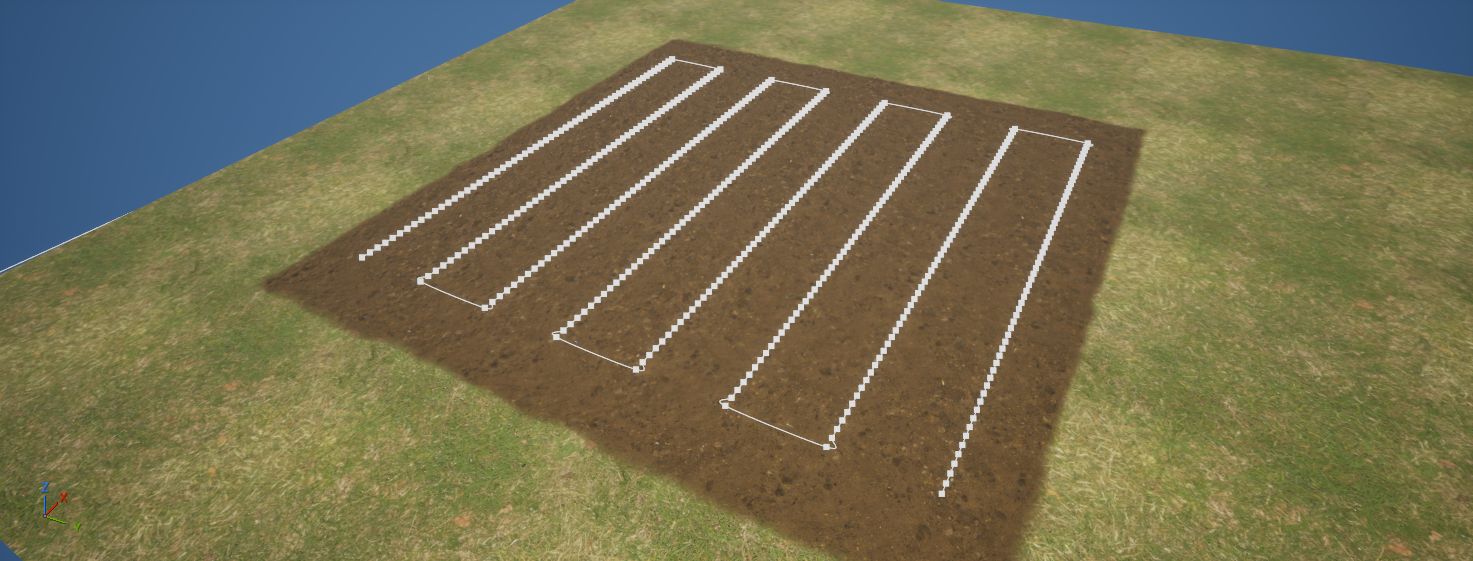
\includegraphics[width=\linewidth]{images/spline_polyline.png}
        \caption{The complete route, defined by individual spline points. The sensor follows this route while capturing images of the scene.}
        \label{splpoly}
    \end{subfigure}\hfill
    \begin{subfigure}{0.48\linewidth}
        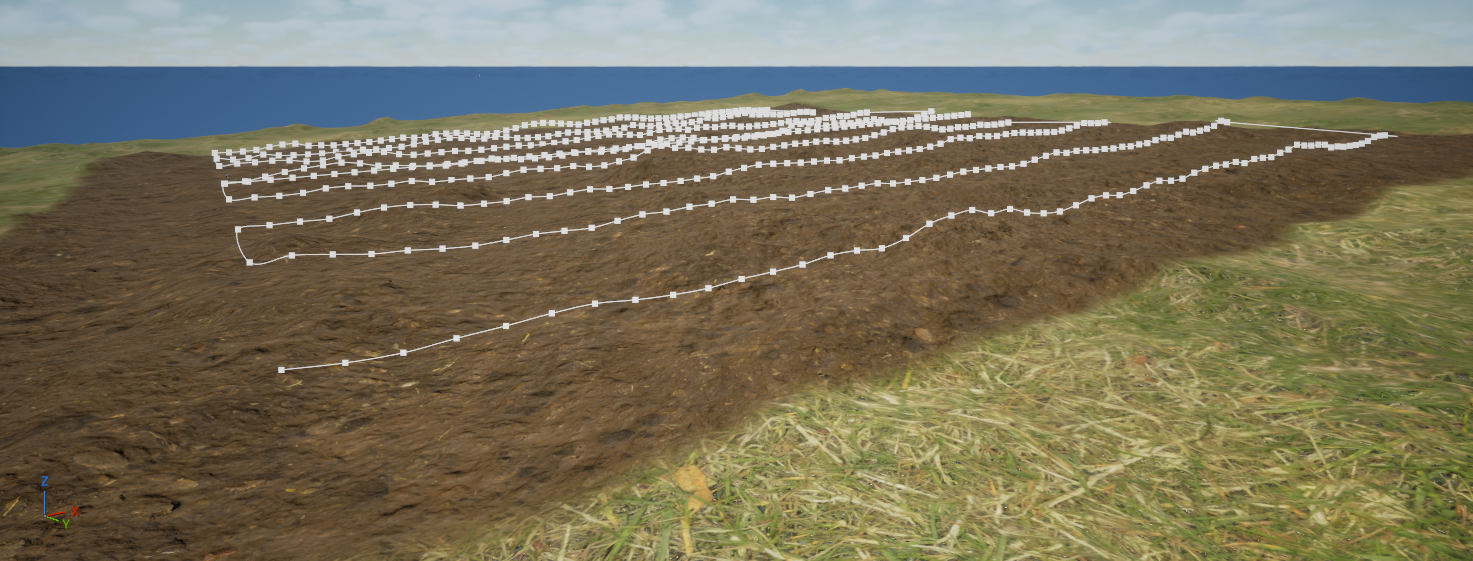
\includegraphics[width=\linewidth]{images/spline_uneven.png}
        \caption{Spline points adapting to the morphology of the ground, making the camera also follow this trail, as if it is mounted onto a vehicle.}
        \label{splunev}
    \end{subfigure}
    
    \caption{Spline points automatically generated based on the dimensions of the field.}
    \label{spline}
\end{figure}


\subsection{Unreal Engine's Sequencer}

Sequencer is a cinematic workflow that allows manipulation of actors. Including a Cine Camera Actor also enables capturing frames of the scene, as the actions described in the Sequencer's actor parameter handling tab are performed. After the parameters are set, rendering can be performed, extracting multiple sequential frames, either in the form of separate images or video.

By adding the aforementioned spline actor to the Sequencer, any actor, in our case the frame-capturing medium, can be attached onto it and follow the path that it defines. This was how SCC was able to traverse the whole field, storing the red and green band luminance of any defined point. It is important to mention that, as discussed in Subsection~\ref{findlum}, using Cine Camera Actor was not possible, despite the amount of tools supporting it within the Sequencer. Although the Cine Camera Actor is capable of rendering linear images, the color it renders is heavily processed, making it incompatible with the light meters' readings.

Sequencer programs the events occurring during the execution of a sequence primarily based on the frames that are programmed to be rendered by a Cine Camera Actor, even if one is not added to the sequence. Therefore, the movement of objects is simulated by defining where each moving object shall be whenever a frame is about to be captured, arranged sequencer events are triggered whenever a frame is about to be captured etc. This was particularly useful for setting up the sampling frequency of the data recording tools, ensuring that SCC captures and actor-position samples were acquired synchronously at a fixed frame-based frequency.

\subsection{Scene Capture Component}

Although Sequencer provides multiple tools dedicated to rendering images using a Cine Camera Actor in an automated fashion, there is a lack of components providing a similar functionality for Scene Capture Components. However, since Sequencer was identified as the most convenient way for simulating the movement of objects, it was necessary to build the data collection around it, even while using SCC as the image rendering medium.

I overcame this problem with the discovery of Frame Capture Manager, a C++ class actor that, as mentioned, makes the ability of SCC to save images to disk visible to other actors. Specifically in this case, the instance of Frame Capture Manager that I added to the digital twin is visible to the Sequencer and, by creating a custom event that triggers at the same rate a Cine Camera would render frames, CaptureNonBlocking is called, collecting automatically the data. The Blueprint of the frame-capturing pipeline is illustrated in Figure~\ref{bluep}.

\begin{figure} [htb]
    \centering
    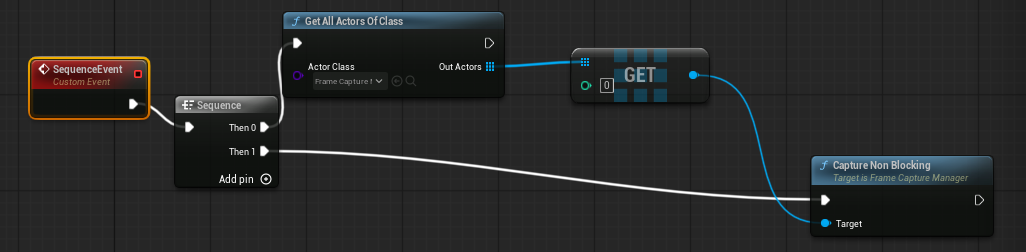
\includegraphics[width=1\linewidth]{images/image.png}
    \caption{Custom event triggering for every programmed frame of the Sequencer. It detects the Frame Capture Manager and calls the function responsible for rendering frames, CaptureNonBlocking. }
    \label{bluep}
\end{figure}

The distance covered by the SCC actor between two separate function calls is fixed. That means that the coordinates of SCC whenever it renders an image remain the same between separate sequences, both when the actor is moving from the start of the spline to its end and the opposite. Consequently, I considered it interesting to also compare GRVI values, as they are measured in these two cases. A simplistic way of achieving this was by setting up the camera's pitch in such a way that the center of its lens is targeted in the middle of the distance between two sequential camera points, essentially calculating the angles of a right triangle whose vertical side is the distance of the camera from the ground and its horizontal side is the distance between the projection of the camera to the ground and the middle of the distance between two consecutive frame-capture positions. It is important to note here that the vertical distance between the camera and the ground was selected instead of the vertical distance between the camera and the field's canopy because the inclusion of the plants' stems, which are more occluded than the canopy, and the field's soil, which, due to its color, adds red-band luminance to the calculated average GRVI of the point of interest, make the model more robust. The pitch of the camera is the angle between the vertical side of the triangle and the hypotenuse, multiplied by negative one ($-1$) (Figure~\ref{camangle}).

\begin{figure} [htb]
    \centering
    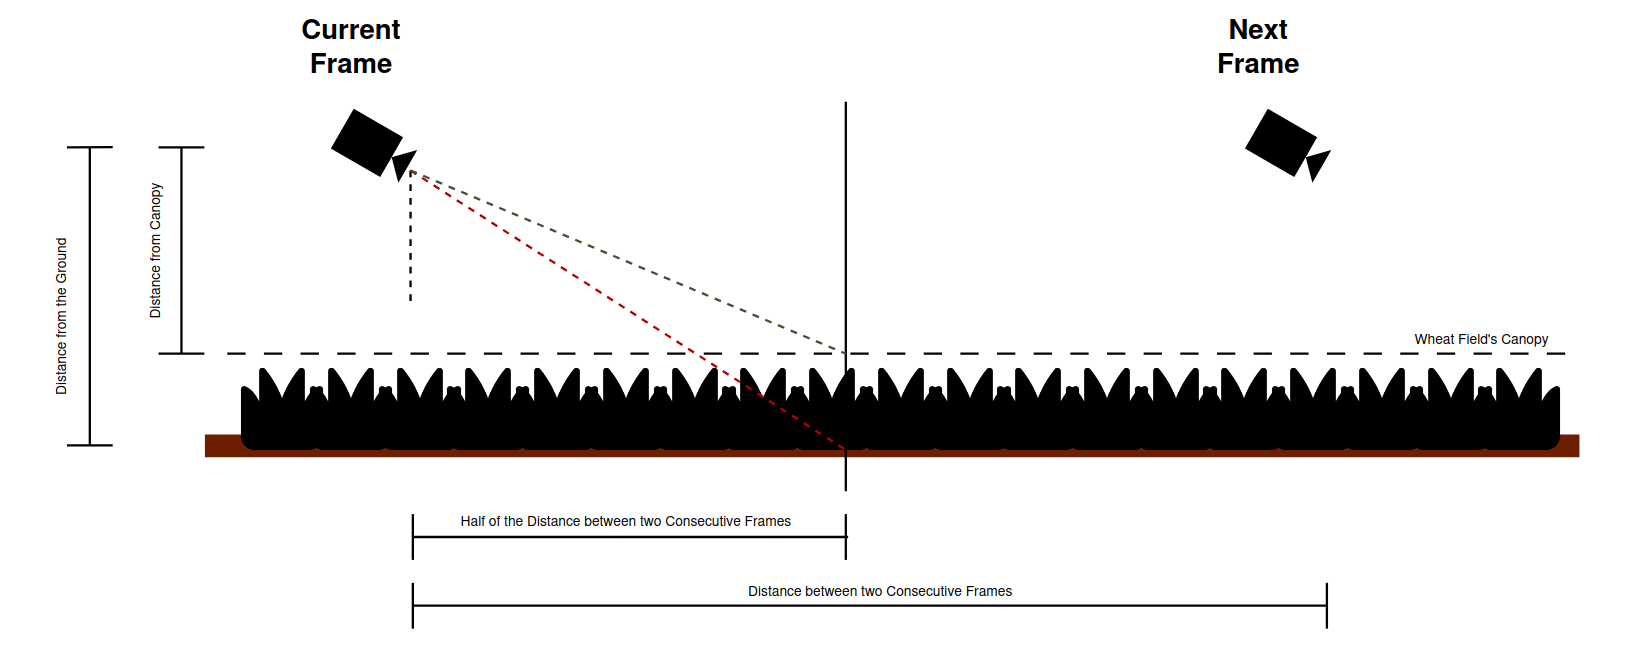
\includegraphics[width=1\linewidth]{images/cameraangle_diag.png}
    \caption{Diagram illustrating how the camera's pitch was calculated. The viewing angle calculated using the distance from the ground is represented by the red dashed line, while the green dashed line represents the angle calculated from the canopy. The first distance captures more comprehensive field data, making the model more robust, and thus was selected.}
    \label{camangle}
\end{figure}

The distance of the SCC from the ground is set to two meters, and the distance between two consecutive frames is approximately 1.4 meters, therefore the sensor's pitch was set to $-20^\circ$. 

\subsection {Light Meters' Position and Readings}

Originally, there were no obstacles between the simulated sun and the field, making the illuminance even across the scene. That meant that a single stationary light meter was sufficient for providing enough information for the whole scene. As an extension of the dataset was developed, including trees that cast shadows over the crop's canopy in several parts of the digital twin, illuminance can differ from point to point. This variance introduced the need to measure illuminance for each examined point of interest. 

To tackle this, I included additional light meters to the project, all attached to the same spline that SSC follows. In a real-world application, the light meters and the camera would be mounted on the same physical rig, making the measurement of the illuminance in the area-of-interest imprecise. Taking advantage of the simulation's lack of physical constraints, the light meters have a slight lead relative to the camera, aiming to measure illuminance directly towards the point where SCC points at. As discussed in (!!!! change this, its moved to the ML parts) \hyperref[feature-engineering]{the Feature Engineering Section}, this simplifying assumption provided the trained models an overly precise context of the illuminance in the studied area, lowering the significance of the relative position of the sun and the camera. (!!!!!!!!!!! this might not be the case!!!!!!!!!) This factor could make the models less transferable to real-world applications. I perform a comparative analysis between the models trained to the data captured with a single light meter placed close to the camera and several light meters placed close to the area-of-interest in the (!!!!!!!!! add hyper-ref here to the chapter-section !!!!!).

Regarding their exact positioning, the light meters were placed approximately in such a distance from the sensor, that their reading corresponds to the center of SCC's field of view, which practically is the middle of the distance between two frames. They are horizontally spread, accounting for the differences in measured illuminance between different parts of the captured scene, considering that it is not guaranteed that either all of the points of interest or none of them will be affected by the shadow of a tree. To avoid repeating the same process with a single light meter attached close to the camera, I took the readings of the central light meter and shifted them backwards, matching each frame with the readings corresponding to the previous frame. Although simplistic, this successfully simulates two important edge cases observed when illuminance is not measured directly on the sensor's field of view: capturing a frame of a shaded surface, while the rig is still exposed to the sun, and the opposite, capturing a frame of an illuminated surface, while the rig is still under the shadow of an obstacle.

In order to store the light meters' readings, I added another Sequencer event. Specifically, each time a frame would be rendered, the measurements, coordinates (so that it can be matched with the appropriate frame) and name of each light meter is printed to UE's render logs. I also developed a PowerShell script, so that when UE's Movie Render Queue is done managing the sequence, the logs are parsed and the printed light meters' information is stored in separate files.

Another assumption that I made regarded the number of included light meters. Although the total number of points of interest per captured frame is twenty, all sharing the same vertical coordinate and being horizontally adjacent to one another, I decided to include only five light meters, each covering four consecutive points of interest. This was mainly implemented in order to avoid overloading the computer hardware resources during Movie Render Queue's execution, considering that for each frame, the information for all added light meter should be read and stored.

\subsection{Solar Zenith Angle and Camera Rotation}

There was one remaining factor for covering the minimum data necessary for providing an ML model a sufficient context of how to interpret the measured GRVI value for a part of the scene and how to approximate its ground truth value through it: the position of the sun relative to the camera's viewing geometry for each frame. Because the solar zenith angle remains constant for each distinct illumination scenario, I logged this metric once per scenario, later to be parsed by a preprocessing script. Camera rotation and coordinates, on the other hand, change from image to image, necessitating the constant recording of this information. By retaining the camera's absolute spatial coordinates when a frame is captured, it is simple to match this frame with the inherent GRVI value of the plants depicted in the frame, assisting with the construction of the noise-free dataset. Simultaneously, tracking the sensor's roll, pitch and yaw provides context about the sun's relative directional orientation at the moment of capture.

In order to achieve that, a Sequencer event quite similar to the one responsible for tracking the light meters' information was developed. This time, during each event trigger, SCC's roll, pitch, yaw and absolute coordinates are printed to the log, which is later parsed, saving the data for the construction of the datasets.

With the completion of this step, the data collection pipeline was finalized. A diagram of this process is illustrated in Figure~\ref{dc-pipe}.


\section{Data Assessment}

\label{datasssessment}

After the render sequences were complete, more than thirty thousand frames were captured. The next step was to evaluate whether they provide meaningful information about the studied phenomena. The primary criteria for the assessment of data were:

\begin{itemize}
    \item Whether SZA affected the perceived GRVI values of the vegetation captured in the frames (Subsection~\ref{sza-aff-grvi}).
    \item How does perceived GRVI behave under overcast lighting and are there differences between the inherent GRVI of distinct materials and their perceived counterparts (Subsection~\ref{diffuse-aff-grvi}).
    \item How do shadows affect GRVI (Subsection~\ref{shadows-aff-grvi}).
\end{itemize}

The answers to these questions served as the primary factors for determining whether the collected data were suitable for subsequent structuring and use in model training.

\begin{figure}[H]
    \centering
    
    \begin{minipage}{1\textwidth}

        \begin{subfigure}{\linewidth}
            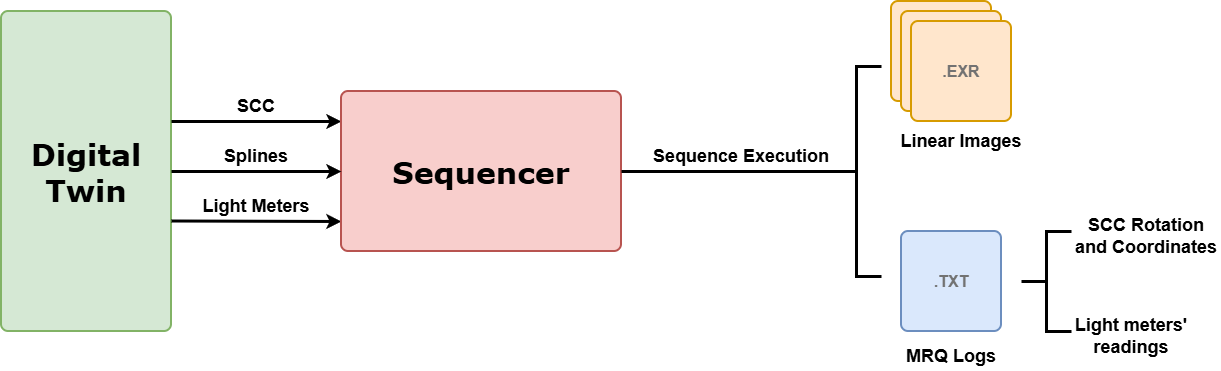
\includegraphics[width=\linewidth]{images/cd-pipe.png}
            \caption{The complete data collection pipeline.}
        \end{subfigure}
        
        \vspace{1em}
        
        \begin{subfigure}{\linewidth}
            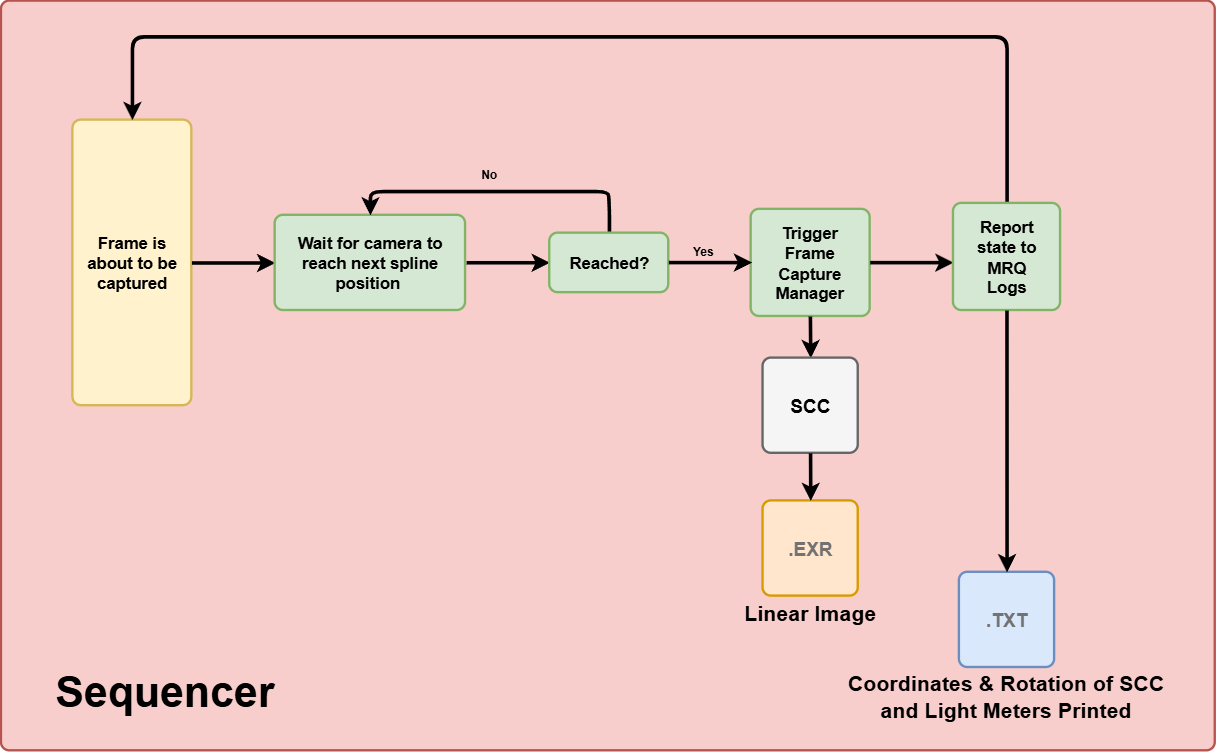
\includegraphics[width=\linewidth]{images/sequencer.png}
            \caption{The steps the sequencer follows for every step of the data collection.}
        \end{subfigure}
        
        \caption{The materials used for the digital twin's terrain, both isolated and combined.}
        \label{dc-pipe}
        
    \end{minipage}
    
\end{figure}

\begin{figure}
    \centering
    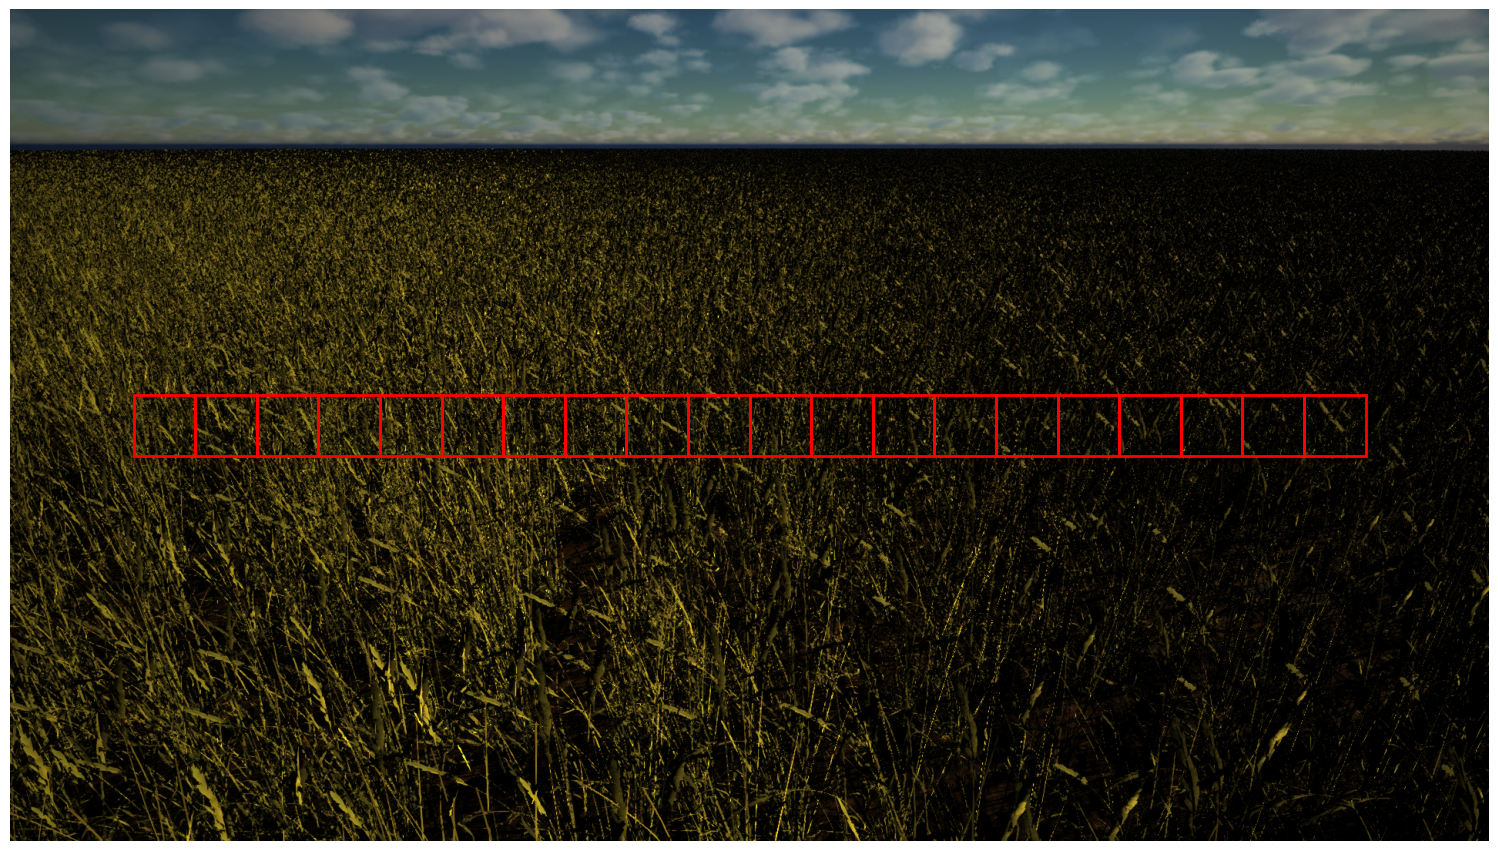
\includegraphics[width=1\linewidth]{images/6_img_lowGRVI.png}
    \caption{areas-of-interest in an image.}
    \label{aoi}
\end{figure}


In addition to the final rendering sequences, I performed several dummy sequences as well, aiming to test the material's properties, isolated from the influence of other materials. Dummy renders differed from the ones  performed for the final data collection by the fact that the SCC was attached to a straight line segment of the developed spline, rather than the full polyline. This was decided in order to examine one case at the time, rather than constantly changing the sun-sensor-canopy geometry. The spline segment was placed in the middle of the digital twin, extending from the lower horizontal bound of the simulated field to the upper one, ensuring that the effects of the SZA variation are not biased towards one side. For all the tests conducted, the areas-of-interest for which the GRVI values were calculated were twenty adjacent square regions arranged horizontally across the image, with a common vertical position corresponding to the vertical center of the frame (Figure~\ref{aoi}).

Another important distinction of the dummy renders is the higher planting density in comparison to the final render sequences. The reasoning behind this was to, at a certain degree, isolate the calculations from the influence of background soil, aiming to observe how each material appears in the scene. That said, parts where soil is visible were kept in an attempt to see how much background soil influences the calculations. Another major reason responsible for the differences in planting density was the difference in the hardware resources needed between dummy and final render sequences. Greater density results in larger overhead. However, dummy renders require significantly less resources due to the presence of fewer actors in the simulation (a grid of crops with different materials applied versus one large crop-block with one material applied) and fewer frames programmed to be captured.

%i can add images of the field during various szas in the addendix

\subsection{SZA Effects on GRVI Values}
\label{sza-aff-grvi}


The behavior of the perceived GRVI values of a field canopy as the SZA changes was one of the primary inspirations for this study. As discussed in Section~\ref{brdf}, a field's canopy





\noindent behaves as an anisotropic reflector. Consequently, depending on the directionality of the incident radiation flux, different amounts of luminance are reflected towards different directions, while the amount of illuminance reaching the surface remains constant. Since the reflectance calculated using the formula for Lambertian surfaces (Equation~\ref{lambertian}) does not account for the directionality of light, as that is a factor that does not affect surfaces that reflect equal amounts of light towards all directions, variations in the SZA cause variations in the calculated reflectance values and, eventually, the calculated GRVI. It was therefore crucial for this study that these variations appear within the digital environment and, most importantly, in the dataset. 

The first test I performed did not include data stored as training examples but rather frames that were captured illustrating the digital twin with only one plant material applied, for multiple materials. The data were captured while SZA was set to $104^\circ$, $-104^\circ$ and $20^\circ$ in sequence, and the green-band illuminance, as measured right above the canopy, was set to 1020. The camera was attached to the straight spline. The primary goal was to confirm that the directionality of light does actually affect perceived reflectance, but also to investigate how different materials are affected. After each data collection was complete, the average GRVI value for each area-of-interest was calculated.

The results were promising, with errors caused by the directionality of the sun being apparent for every material I tested. Interestingly enough, depending on the inherent GRVI values of the material, the effects of SZA variation were quite different. In Figure~\ref{highgrvigrid} for example, a relatively high GRVI material (the highest appearing in the GRVI map, being 0.38) was set to the digital twin's meshes. Setting the SZA to $-104^\circ$ resulted in the right half of the field appearing more occluded than the left (Figure~\ref{6highimg}). This effect was also represented in the average GRVI per area-of-interest graphs, with the occluded part having overall lower GRVI values than the rest (Figure~\ref{6highgraph}). Specifically, the graph exhibits a downward trend towards the edge of the occluded region, with the boundary-adjacent area-of-interest exhibiting the lowest GRVI value. Similar results were observed when setting the SZA to $104^\circ$. This time, the left part of the field was occluded, having overall lower GRVI values. 

\begin{figure}[htb]
    \centering

    \begin{subfigure}{0.3\textwidth}
        \centering
        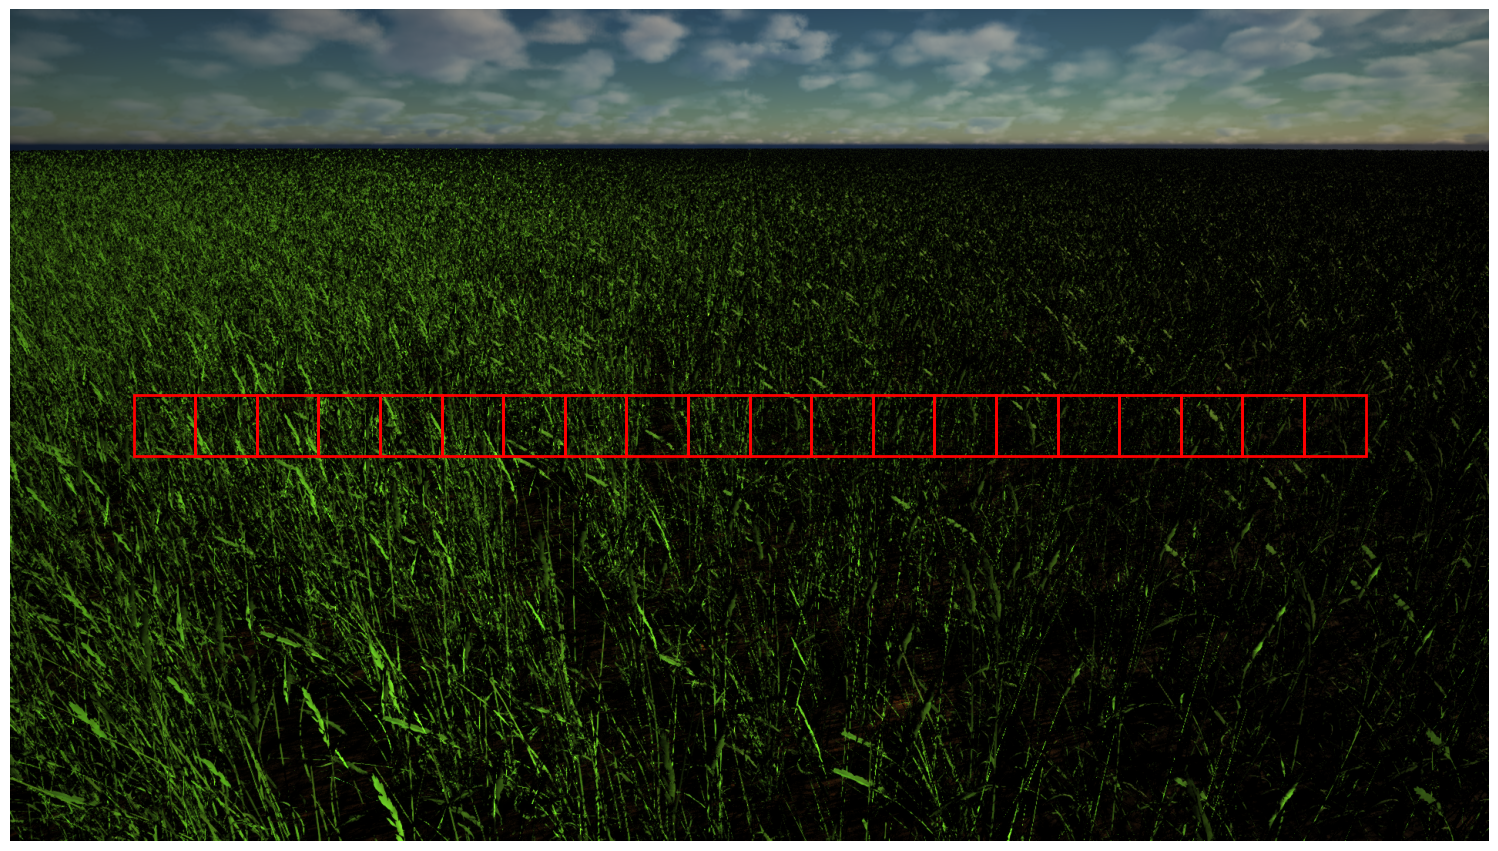
\includegraphics[width=\linewidth]{images/6_img_highGRVI.png}
        \caption{$-104^\circ$}
        \label{6highimg}
    \end{subfigure}
    \hfill
    \begin{subfigure}{0.3\textwidth}
        \centering
        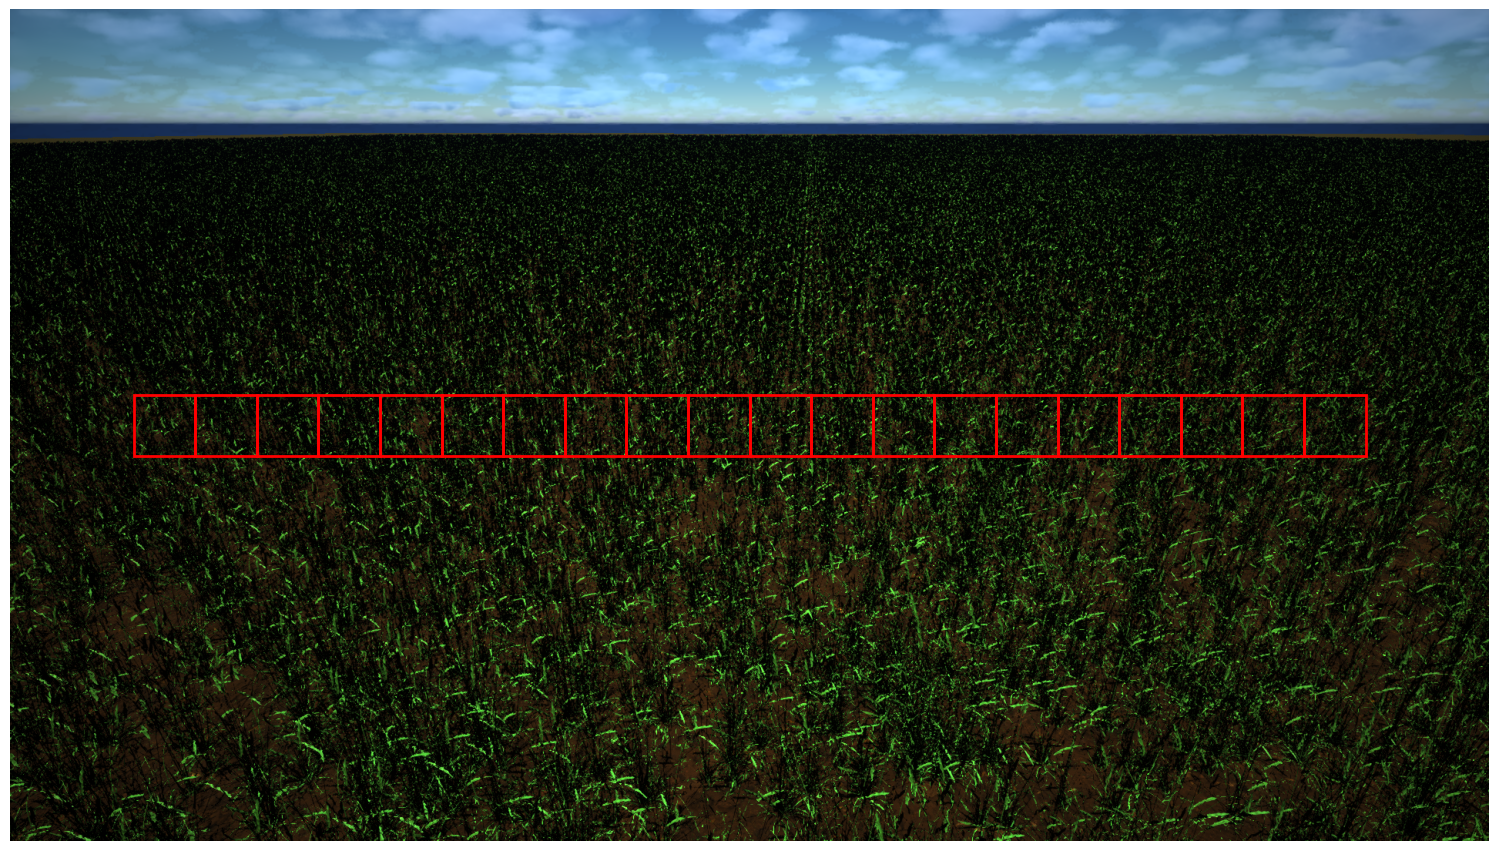
\includegraphics[width=\linewidth]{images/12_img_highGRVInc.png}
        \caption{$20^\circ$}
        \label{12highimg}
    \end{subfigure}
    \hfill
    \begin{subfigure}{0.3\textwidth}
        \centering
        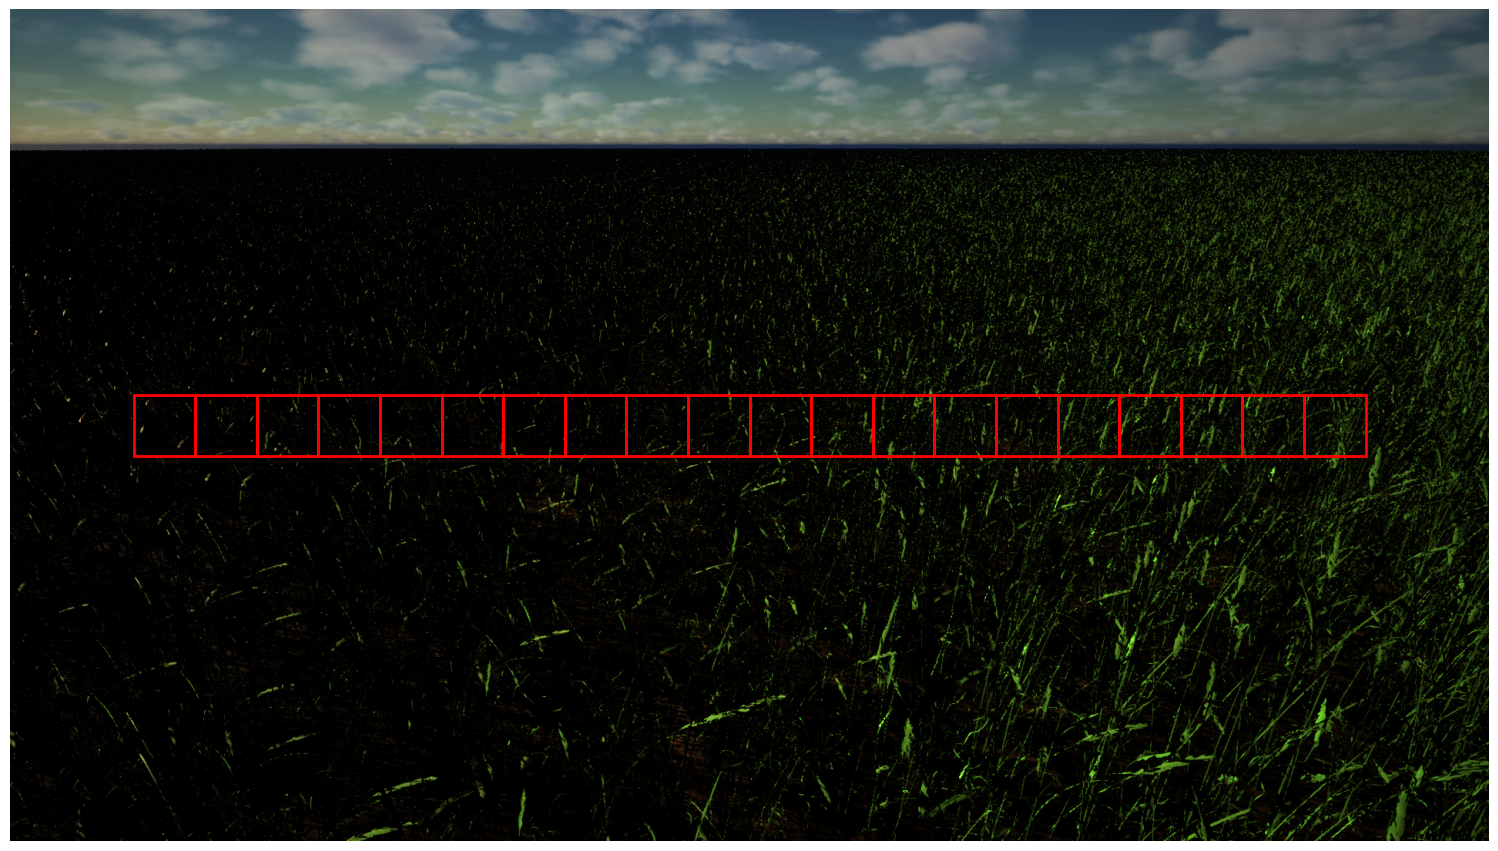
\includegraphics[width=\linewidth]{images/1715_img_highGRVI.png}
        \caption{$104^\circ$}
        \label{1715highimg}
    \end{subfigure}

    \vspace{0.5cm}

    \begin{subfigure}{0.3\textwidth}
        \centering
        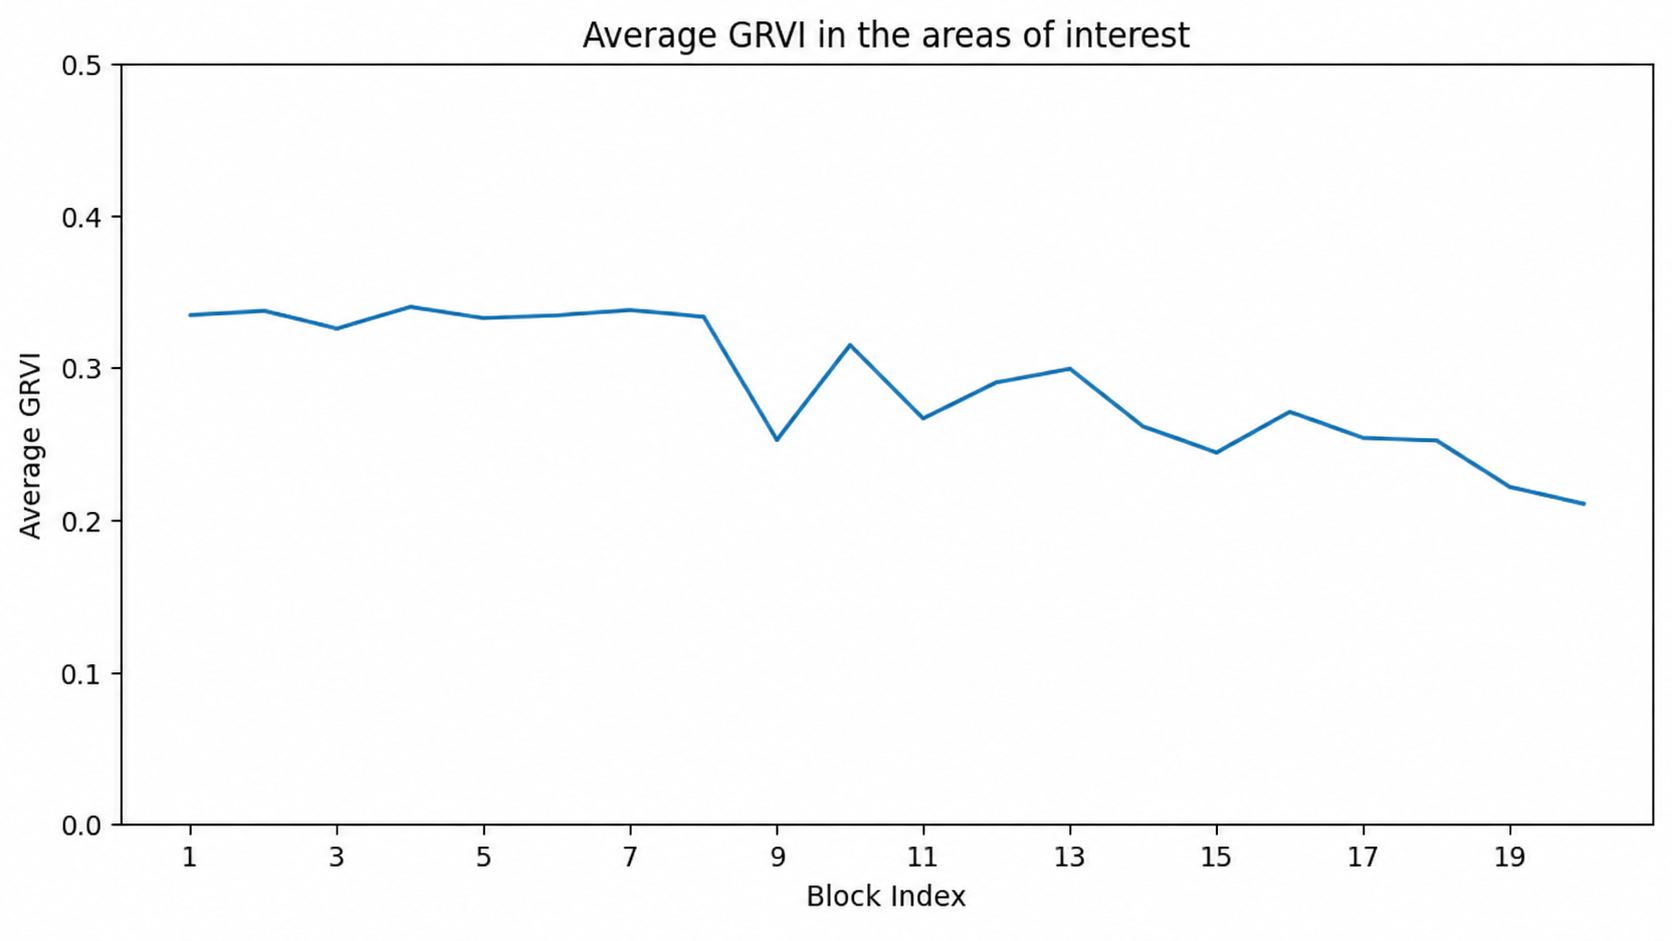
\includegraphics[width=\linewidth]{images/6_graph_highGRVI.png}
        \caption{$-104^\circ$}
        \label{6highgraph}
    \end{subfigure}
    \hfill
    \begin{subfigure}{0.3\textwidth}
        \centering
        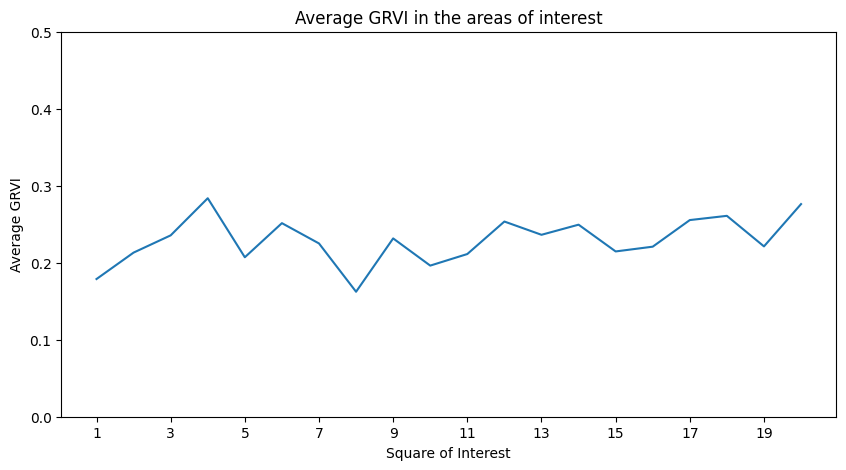
\includegraphics[width=\linewidth]{images/12_graph_highGRVInc.png}
        \caption{$20^\circ$}
        \label{12highgraph}
    \end{subfigure}
    \hfill
    \begin{subfigure}{0.3\textwidth}
        \centering
        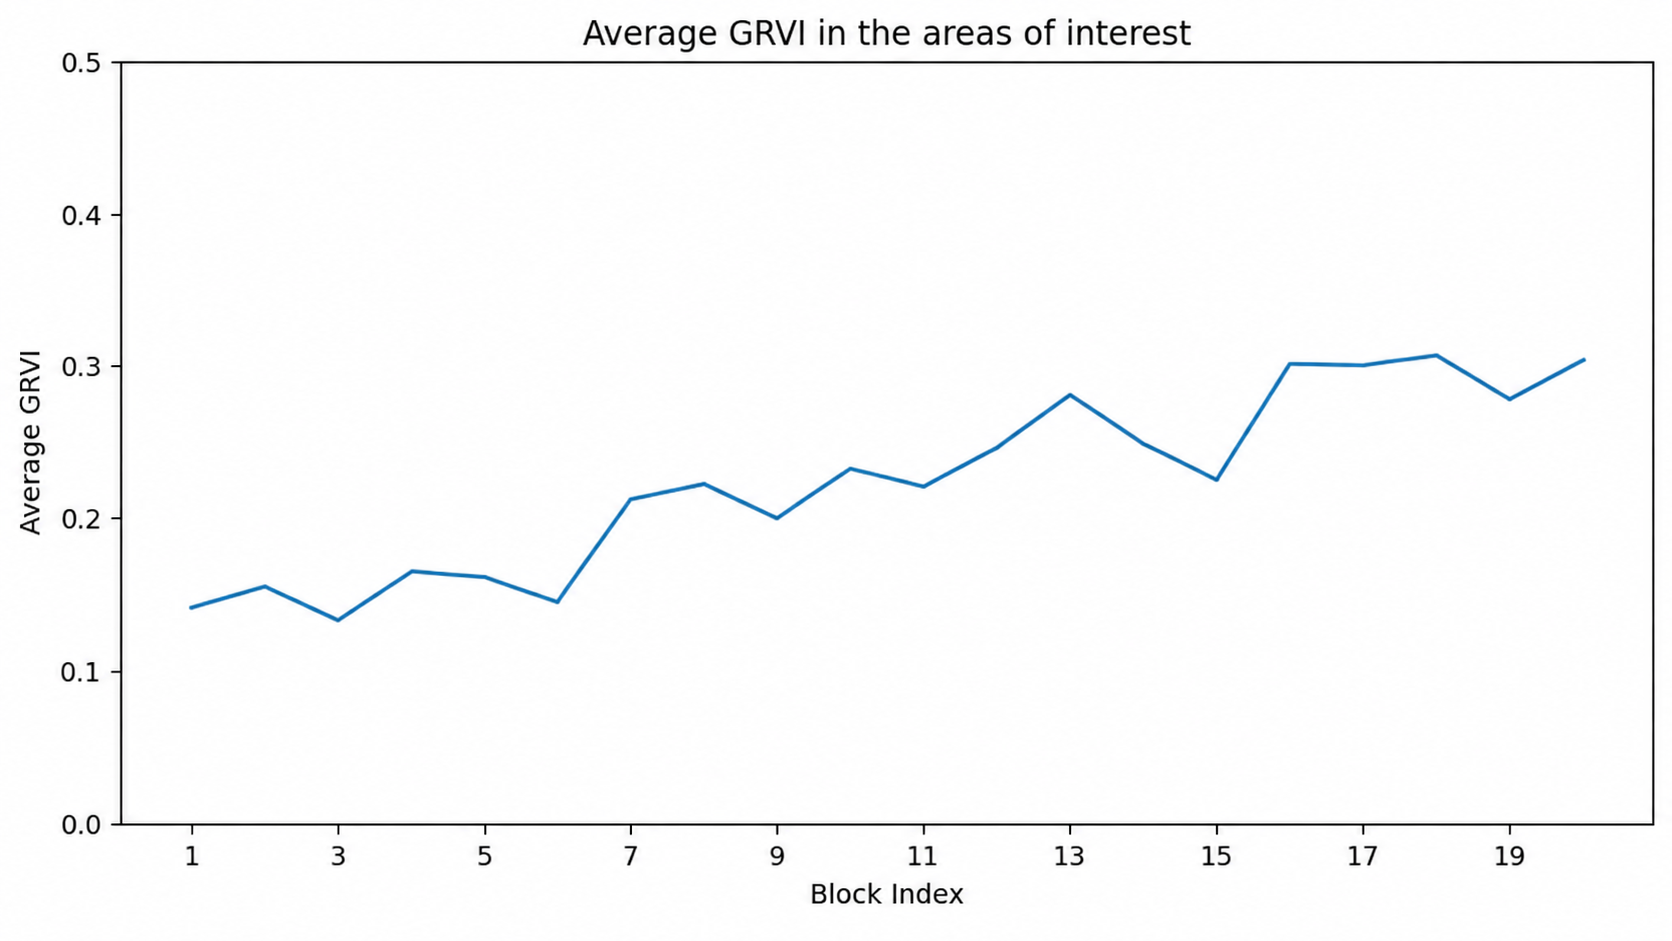
\includegraphics[width=\linewidth]{images/1715_graph_highGRVI.png}
        \caption{$104^\circ$}
        \label{1715highgraph}
    \end{subfigure}

    \caption{Images captured under various SZAs. The red squares indicate the bounds of the areas-of-interest. The corresponding graphs present the mean GRVI calculated for the same indexed areas-of-interest across all captured frames. The material used for the illustrated plants has an inherent GRVI of 0.38.}
    \label{highgrvigrid}
\end{figure}

The average values of the images captured with SZA set to $20^\circ$ manage to depict several of the rest of the factors that introduce noise to the measurements, including the uneven planting density of the crops, which results in more soil being visible and, consequently, dips in the average GRVI (for instance, in areas-of-interest with index 5 and 8 in Figure~\ref{12highimg}), and the dependency on the camera viewing geometry. Since the directional light is not angled, we see that there is no downward trend in the GRVI graph towards one of the sides of the image, the way it occurs for the other two cases ($-104^\circ$ and $104^\circ$).

The exact opposite results were observed while conducting the same experiments using low GRVI materials regarding the effects of SZA. As illustrated in Figure~\ref{lowgrvigrid}, this time GRVI values follow an upward trend within the occluded region, with a way smaller absolute difference between the GRVI values rightmost and leftmost. This time, the average GRVI values for SZA equal to $20^\circ$ were barely above the highest value recorded in the occluded part of the field (Figure~\ref{12lowgraph}.

\begin{figure}[htb]
    \centering

    \begin{subfigure}{0.3\textwidth}
        \centering
        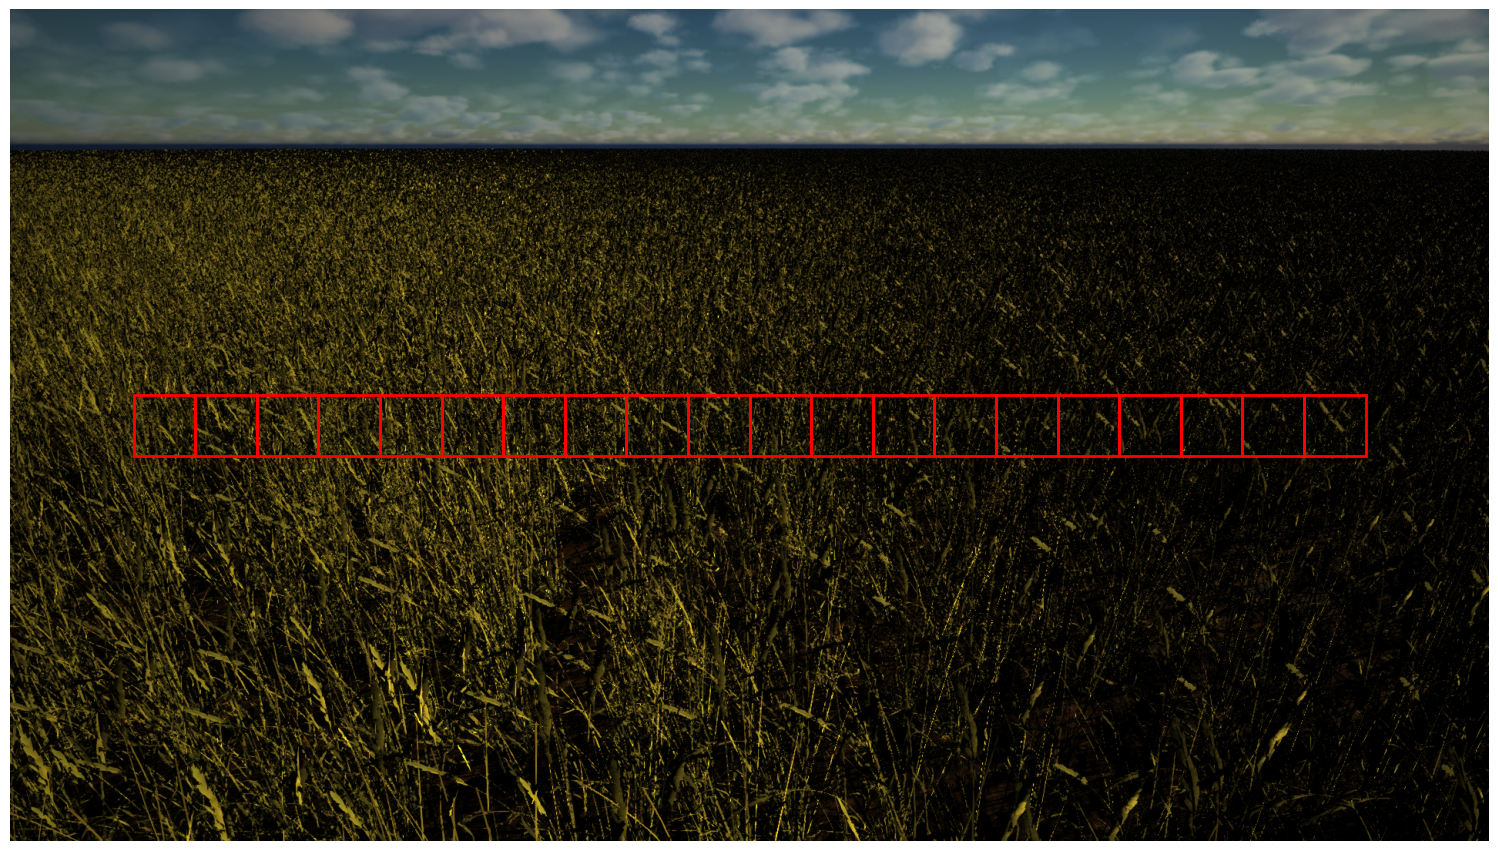
\includegraphics[width=\linewidth]{images/6_img_lowGRVI.png}
        \caption{$-104^\circ$}
        \label{6lowimg}
    \end{subfigure}
    \hfill
    \begin{subfigure}{0.3\textwidth}
        \centering
        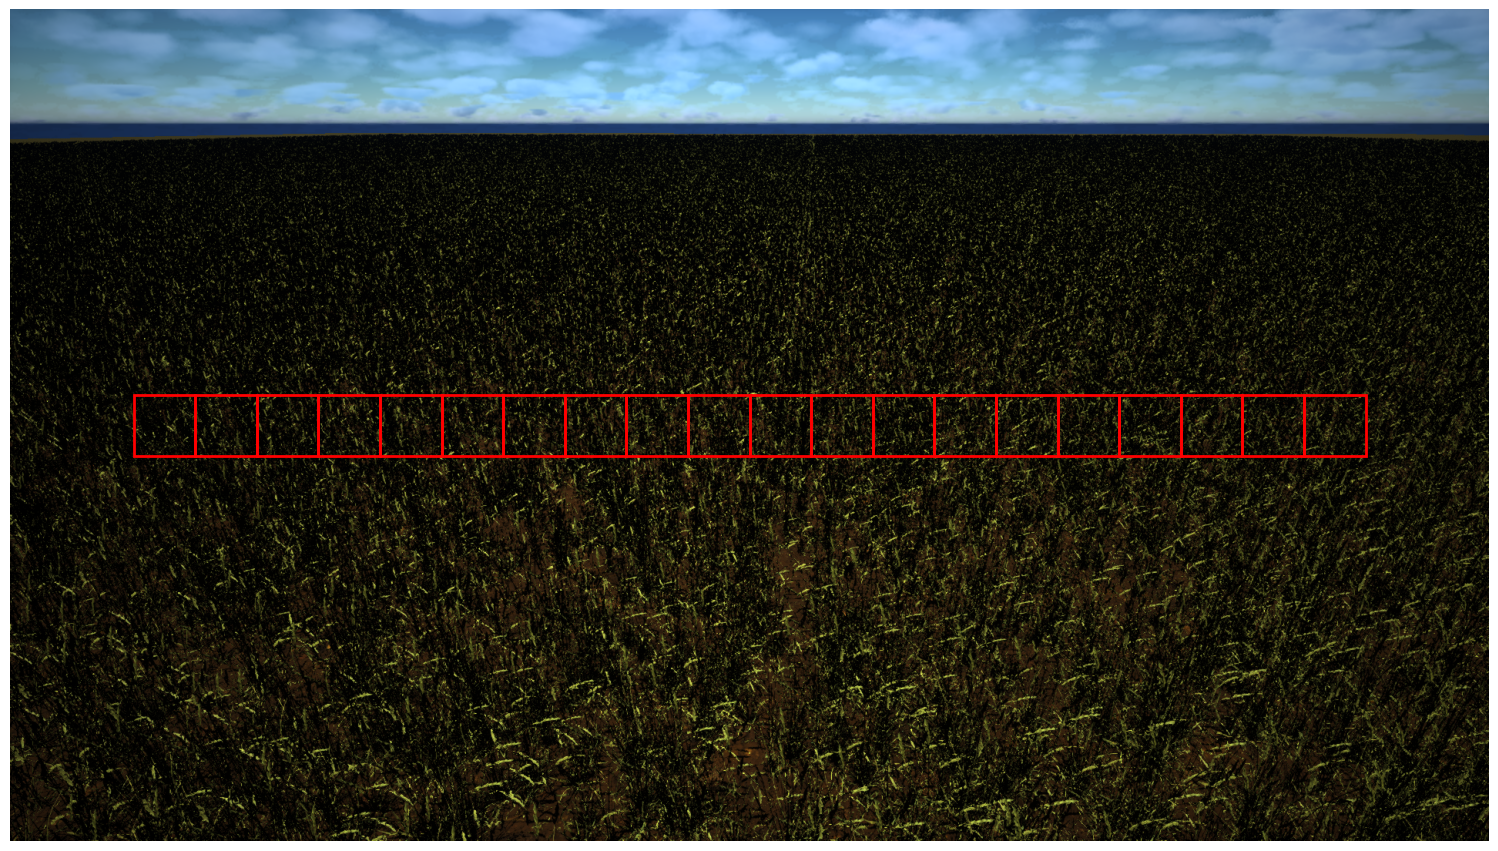
\includegraphics[width=\linewidth]{images/12_img_lowGRVInc.png}
        \caption{$20^\circ$}
        \label{12lowimg}
    \end{subfigure}
    \hfill
    \begin{subfigure}{0.3\textwidth}
        \centering
        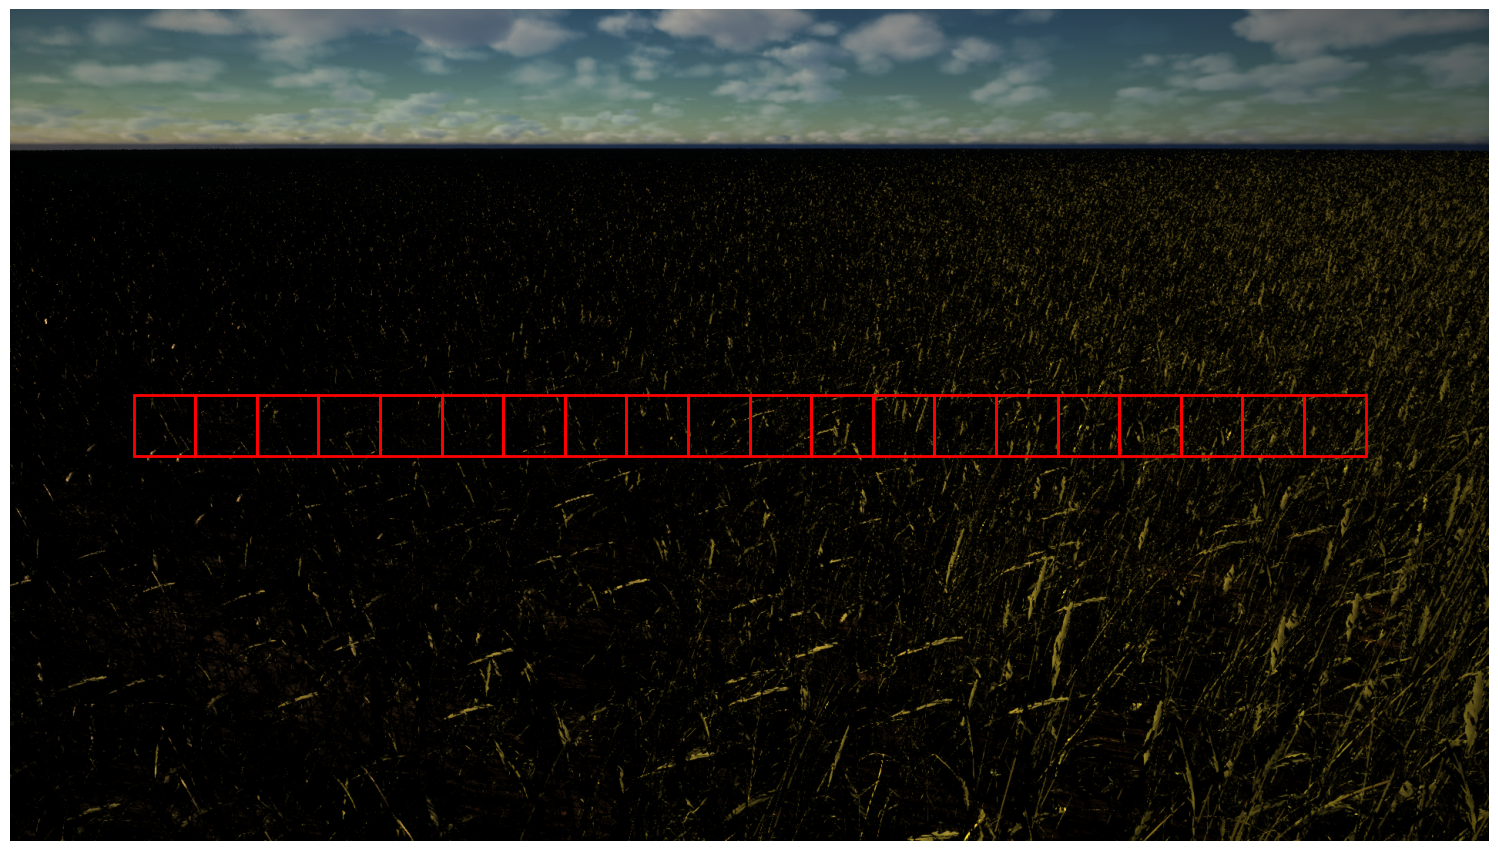
\includegraphics[width=\linewidth]{images/1715_img_lowGRVI.png}
        \caption{$104^\circ$}
        \label{1715lowimg}
    \end{subfigure}

    \vspace{0.5cm}

    \begin{subfigure}{0.3\textwidth}
        \centering
        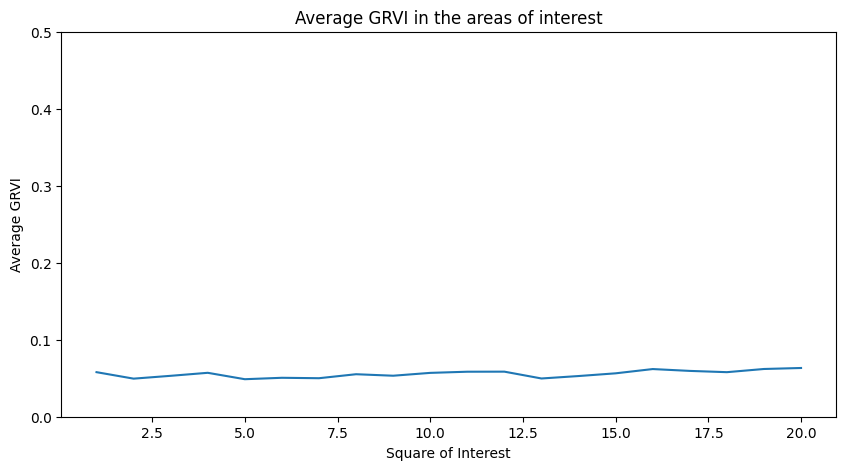
\includegraphics[width=\linewidth]{images/6_graph_lowGRVI.png}
        \caption{$-104^\circ$}
        \label{6lowgraph}
    \end{subfigure}
    \hfill
    \begin{subfigure}{0.3\textwidth}
        \centering
        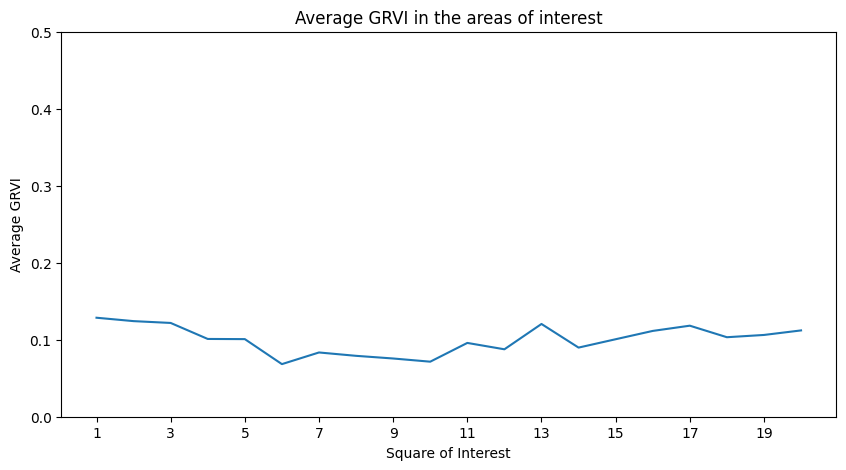
\includegraphics[width=\linewidth]{images/12_graph_lowGRVInc.png}
        \caption{$20^\circ$}
        \label{12lowgraph}
    \end{subfigure}
    \hfill
    \begin{subfigure}{0.3\textwidth}
        \centering
        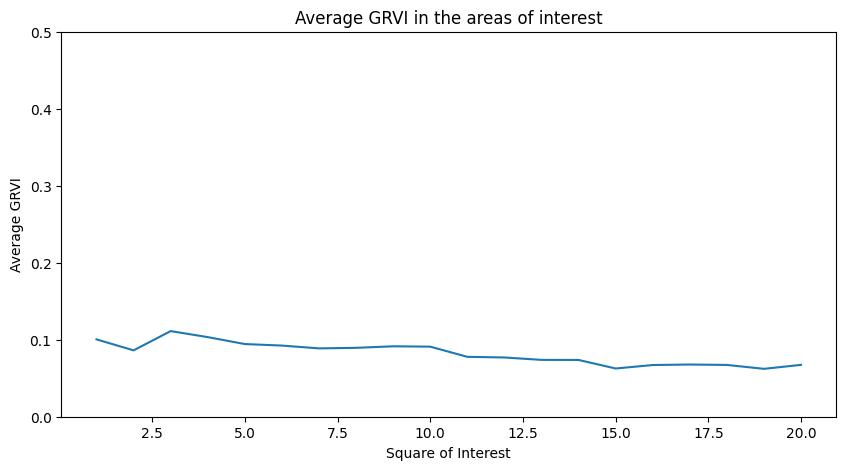
\includegraphics[width=\linewidth]{images/1715_graph_lowGRVI.png}
        \caption{$104^\circ$}
        \label{1715lowgraph}
    \end{subfigure}

    \caption{Images captured under various SZAs. The red squares indicate the bounds of the areas-of-interest. The corresponding graphs present the mean GRVI calculated for the same indexed areas-of-interest across all captured frames. The material used for the illustrated plants has an inherent GRVI of 0.08.}
    \label{lowgrvigrid}
\end{figure}

Overall, for all the materials I tested, there was a similar pattern observed: all bright-appearing parts of the images have roughly the same perceived GRVI value, with fluctuations caused by the viewing geometry, presence of soil and more, while measurements regarding the occluded part of the field follow an upward or downward trend towards the edge of the occluded region, depending on the material. To measure how much each material is affected  by the directionality of light, I used the percentile difference between the edge of the occluded part and the edge of the bright-appearing region:

\begin{equation}
    \%Diff = \frac{GRVI_O - GRVI_B}{GRVI_B}
    \label{nonsymDiff}
\end{equation}

With the SZA fixed at $104^\circ$ and green-band illuminance equal to 1020, the occluded part appears at the left side of the scene. The results of the measurements are illustrated in Figure~\ref{graphComp}.

\begin{figure} [htb]
    \centering
    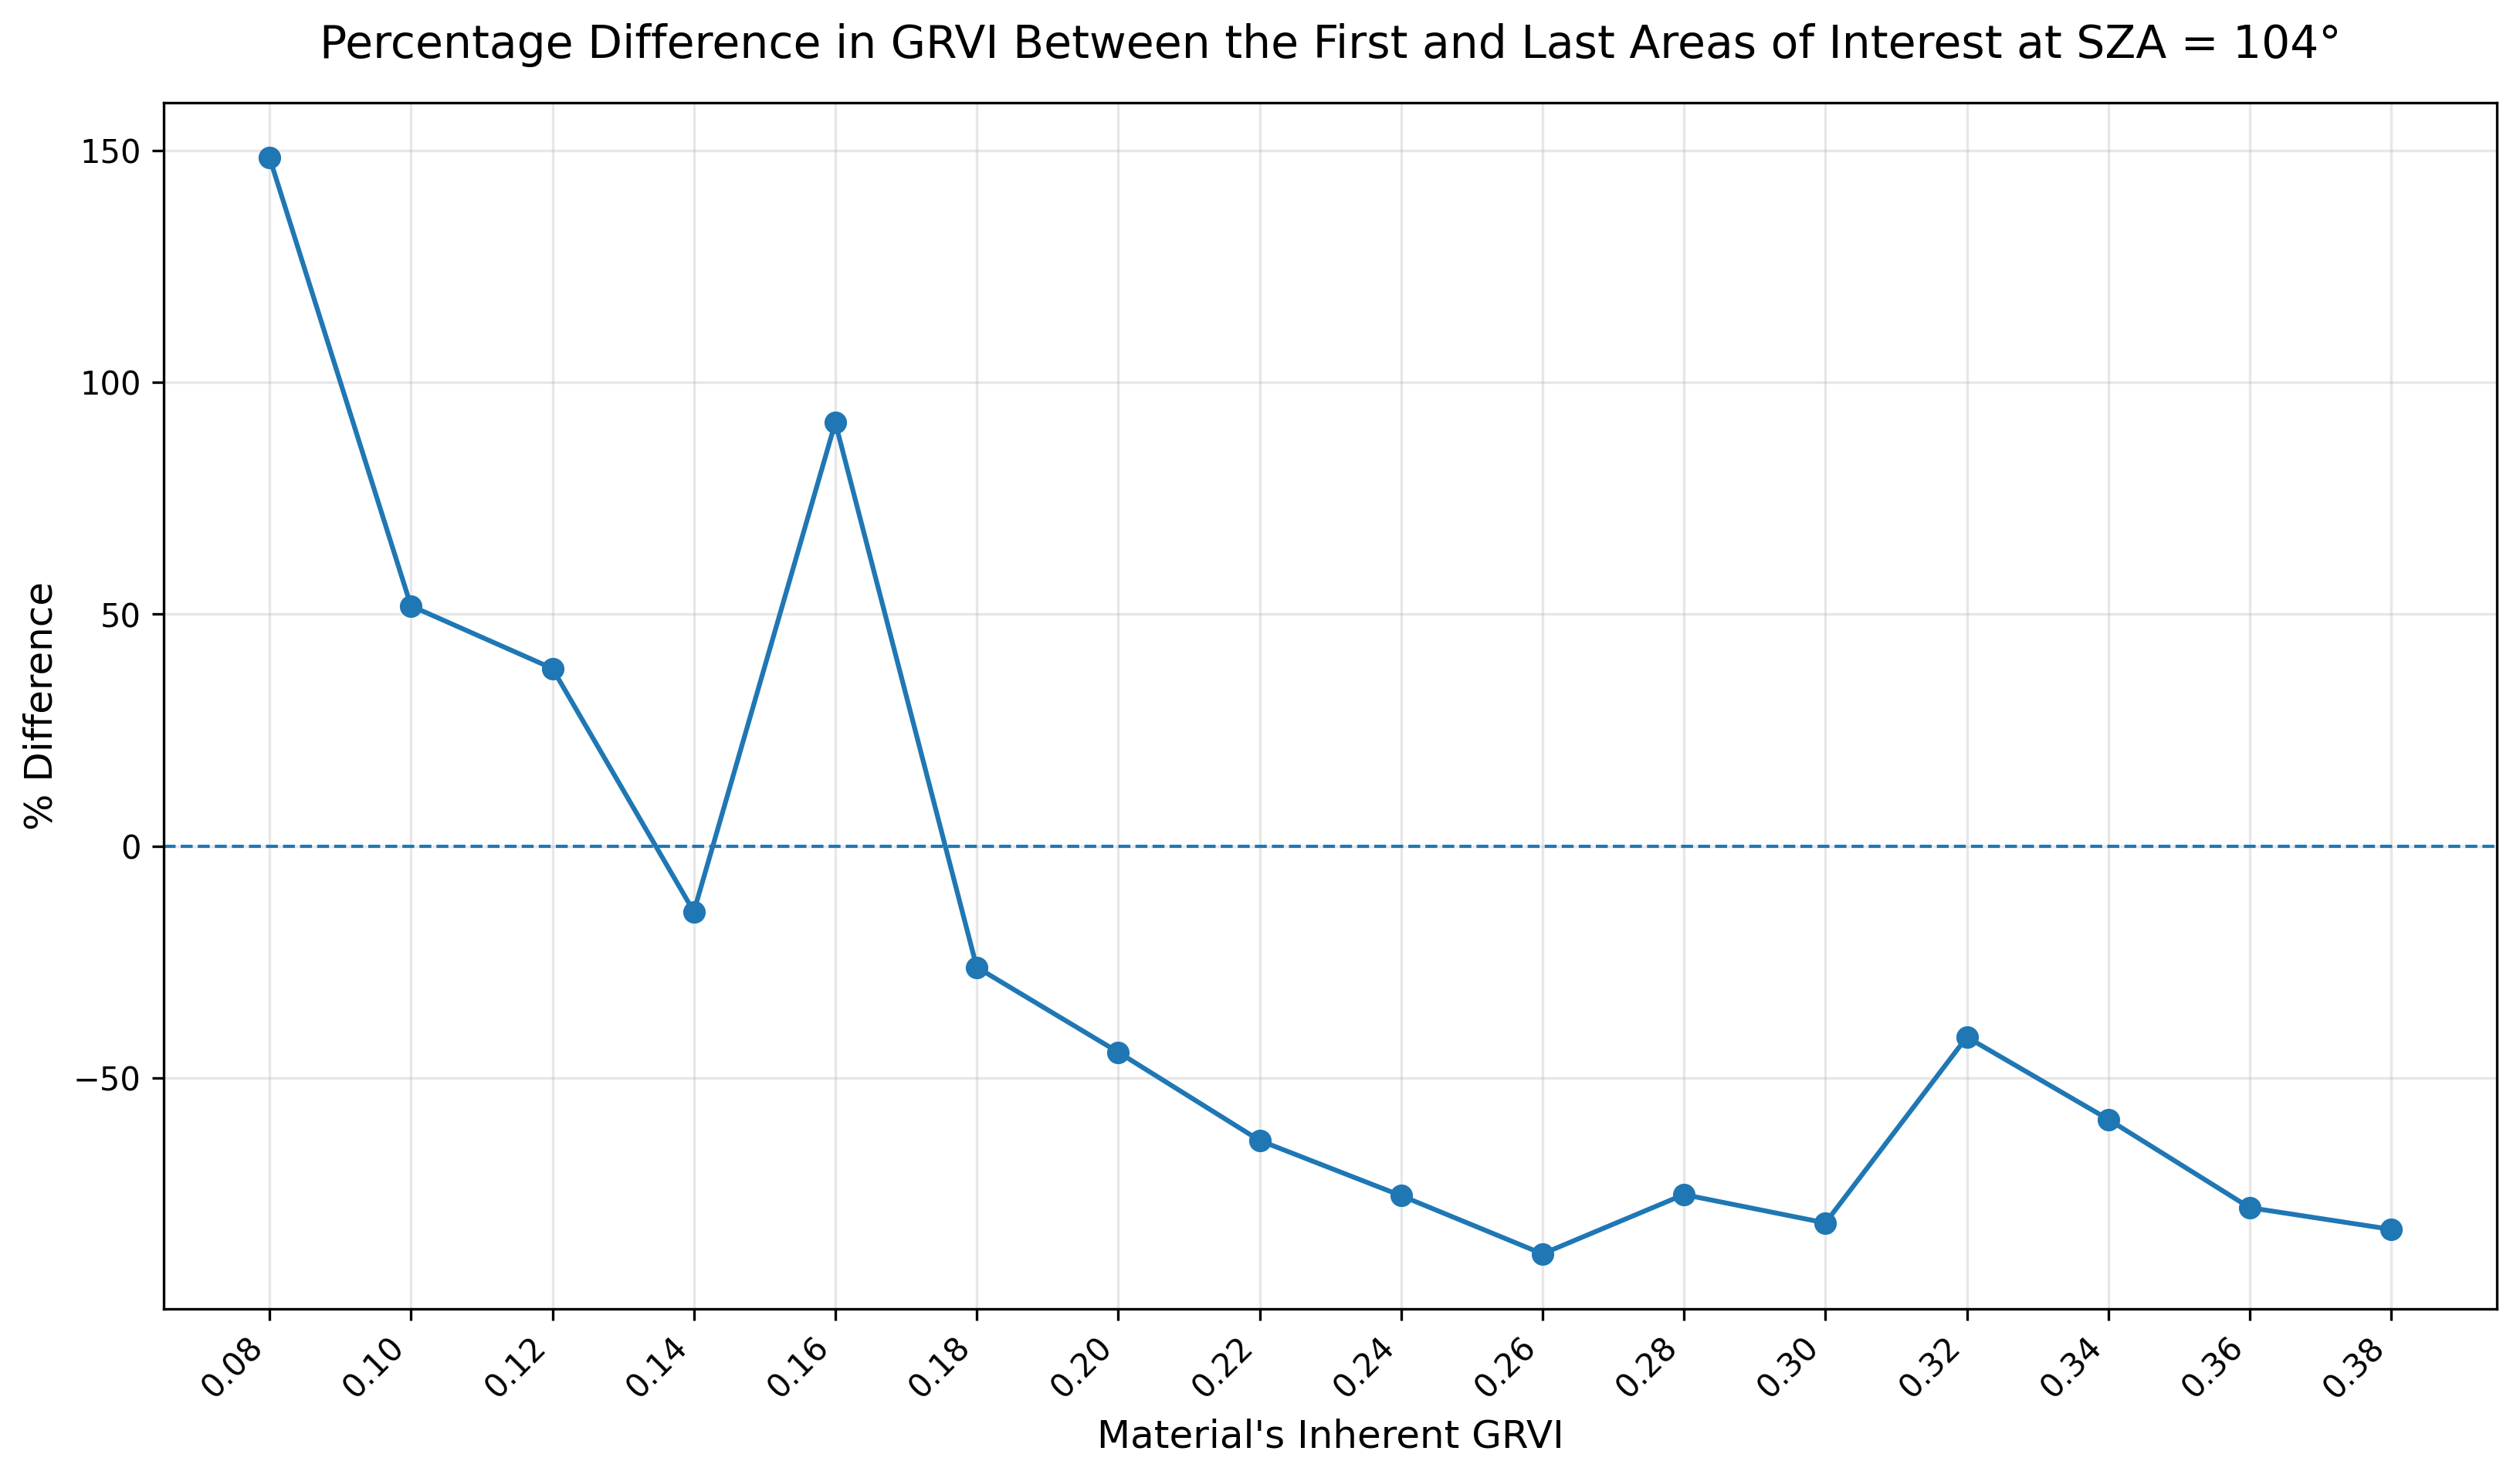
\includegraphics[width=1\linewidth]{images/grvi_percentage_difference_sza_104.png}
    \caption{Average Percentage difference between the rightmost and leftmost areas-of-interest of the captured images. Since the SZA was set to $104^\circ$, the first belongs to the bright-appearing region of the field, while the latter belongs to the occluded region of the frames.}
    \label{graphComp}
\end{figure}

The next test regarded the differences between two separate render sequences, one performed with SZA set to $-104^\circ$ and one with SZA set to $104^\circ$. Green-band illuminance remained at 1020. This time, the data collected from the final render sequences were used. The comparison was made between the areas-of-interest of the frames captured while SZA was set to $104^\circ$ and the areas-of-interest of their matching frames captured while SZA was set to $-104^\circ$. The difference between the measured values was expressed with the symmetric percent difference:

\begin{equation}
    \%Diff = \frac{|GRVI_{104} - GRVI_{-104}|}{\frac{|GRVI_{104}| + |GRVI_{-104}|}{2}}
    \label{symDiff}
\end{equation}


Whenever the difference between two areas-of-interest with the same index was calculated, the percentage was added to a common total for the specific index. By the end of the process, I divided the total for each index with the number of compared frames, resulting in the mean percentage difference for the specific index across the dataset. As discussed in Section~\ref{DC}, since during the final render sequences SCC follows a path defined by a spline that forms an orthogonal polyline traversing the whole field, the sun-canopy-sensor geometry changes over time. However, this should not affect the symmetric difference as long as the sensor's yaw remains either $0^\circ$ or $180^\circ$. I excluded cases where the sensor's yaw is neither $0^\circ$ nor $180^\circ$, since they are not part of this study.

\begin{figure} [htb]
    \centering
    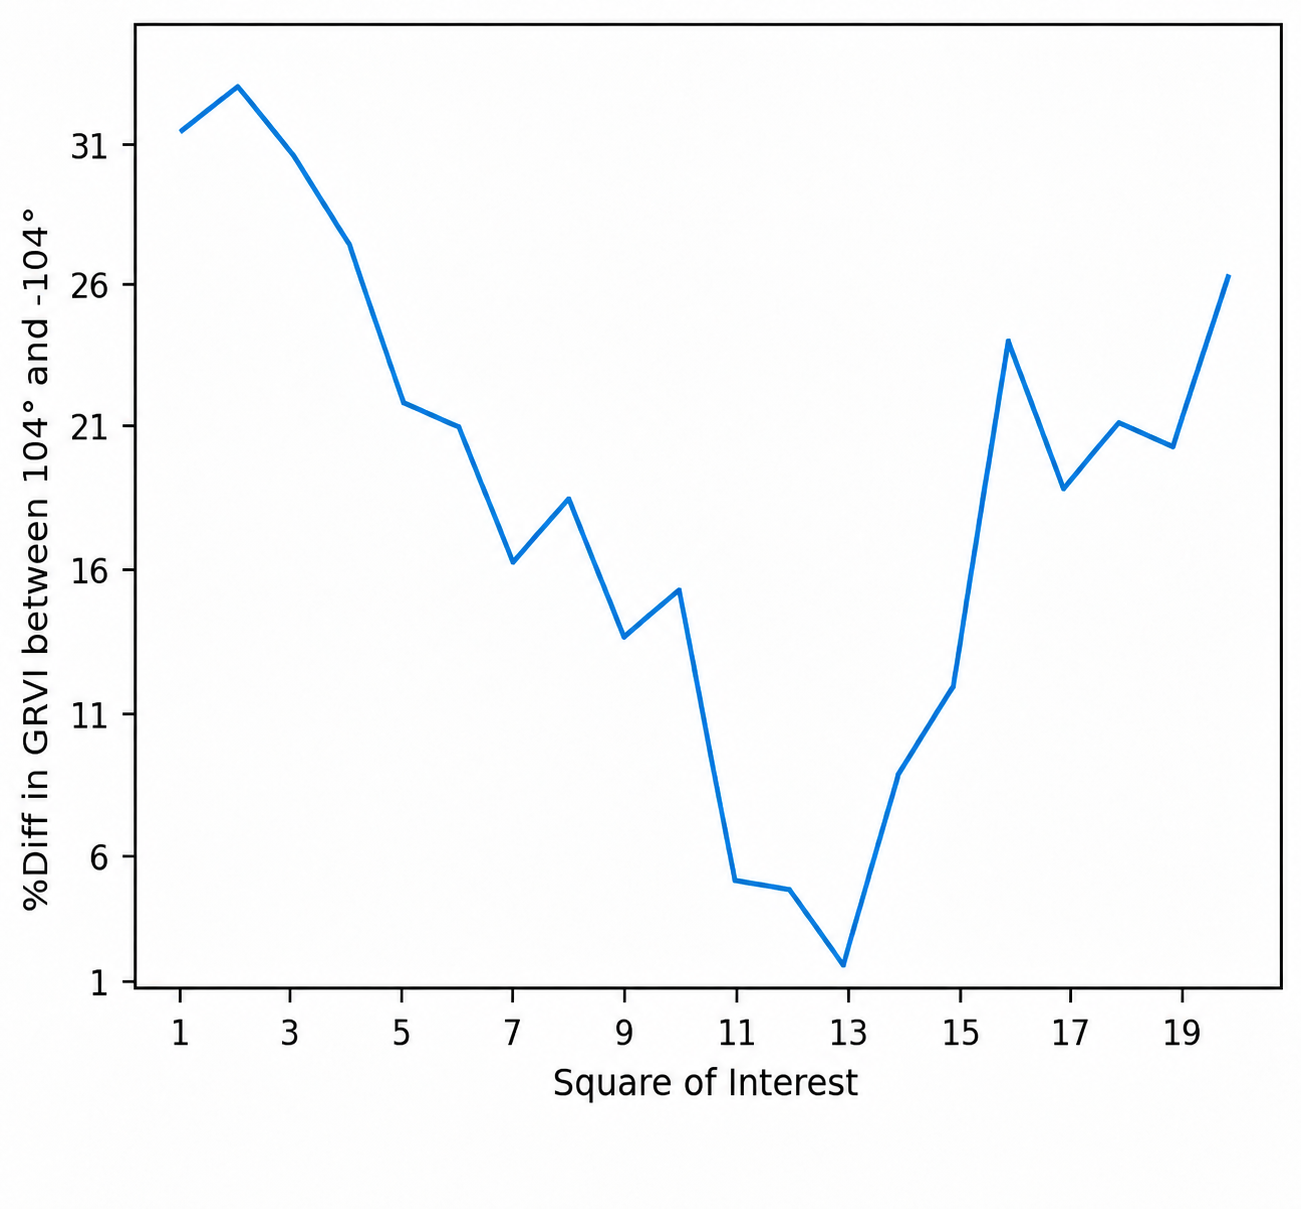
\includegraphics[width=1\linewidth]{images/104-104grviDiff.png}
    \caption{Average percentage difference between frames captured with SZA set to $104^\circ$ and $-104^\circ$. Comparisons are performed between corresponding areas-of-interest with the same frame index and the same within-frame index across different render sequences}
    \label{104-104}
\end{figure}

The results of this experiment are depicted in Figure~\ref{104-104}. As shown, areas closer to the bounds of the frame tend to differ more than areas closer to the middle. The reason behind that is that, closer to the middle, there is an overlapping region for both of the angles with equal magnitude and opposite signs, where the field appears almost equally bright. Consequently, percentage difference in this region is relatively low. On the other hand, regions closer to the bounds appear bright for one of the  cases and occluded for the other, with the difference becoming more evident as we approach the edge.

With these tests complete, it is apparent that the studied phenomenon of directional reflectance is well represented within the digital environment and captured during the data collection.

\subsection{GRVI under Diffuse Lighting Conditions}
\label{diffuse-aff-grvi}


As mentioned in \hyperref[chap1]{the Introduction}, cloudy weather's ability to mitigate directional light has been exploited by researchers as a way of acquiring consistent radiometric measurements, without the errors introduced by shadows and the crops' canopy behaving as an anisotropic reflector. That said, these factors are not the only sources of error affecting the perceived GRVI. In order to investigate further sources of error, the next experiments I conducted within the digital twin regarded analyzing information captured under overcast lighting conditions. This experimentation aimed to uncover whether data collected under such conditions could be used as a reference baseline, capable of mitigating the more prominent sources of noise, or just as a temporary solution, aiming to isolate the measurements from the effects of the light's directionality, before a subsequent method is applied.

Following a testing pipeline similar to that of the previous subsection, the first experiment examined the GRVI values calculated when a single material is applied to the simulated field, this time under overcast lighting conditions. Specifically, I performed a dummy render sequence for each of the inherent GRVI values present on Table~\ref{diff-griv-field}, with SCC's yaw fixed to $0^\circ$, SZA set to $20^\circ$ and non-zero Mie Scattering Scale applied. I avoided presenting average value graphs (similar to the ones presented in \ref{highgrvigrid}) for this experiment, as it is important for the noise present in single examples not to be suppressed. Instead, I selected multiple examples per render sequence stochastically, aiming to address possible errors responsible for the non-uniform perceived GRVI of the scene, despite the absence of directional light. Several examples are illustrated in Figure~\ref{cloudy-grid}

\begin{figure}[htb]
    \centering

    \begin{subfigure}{0.3\textwidth}
        \centering
        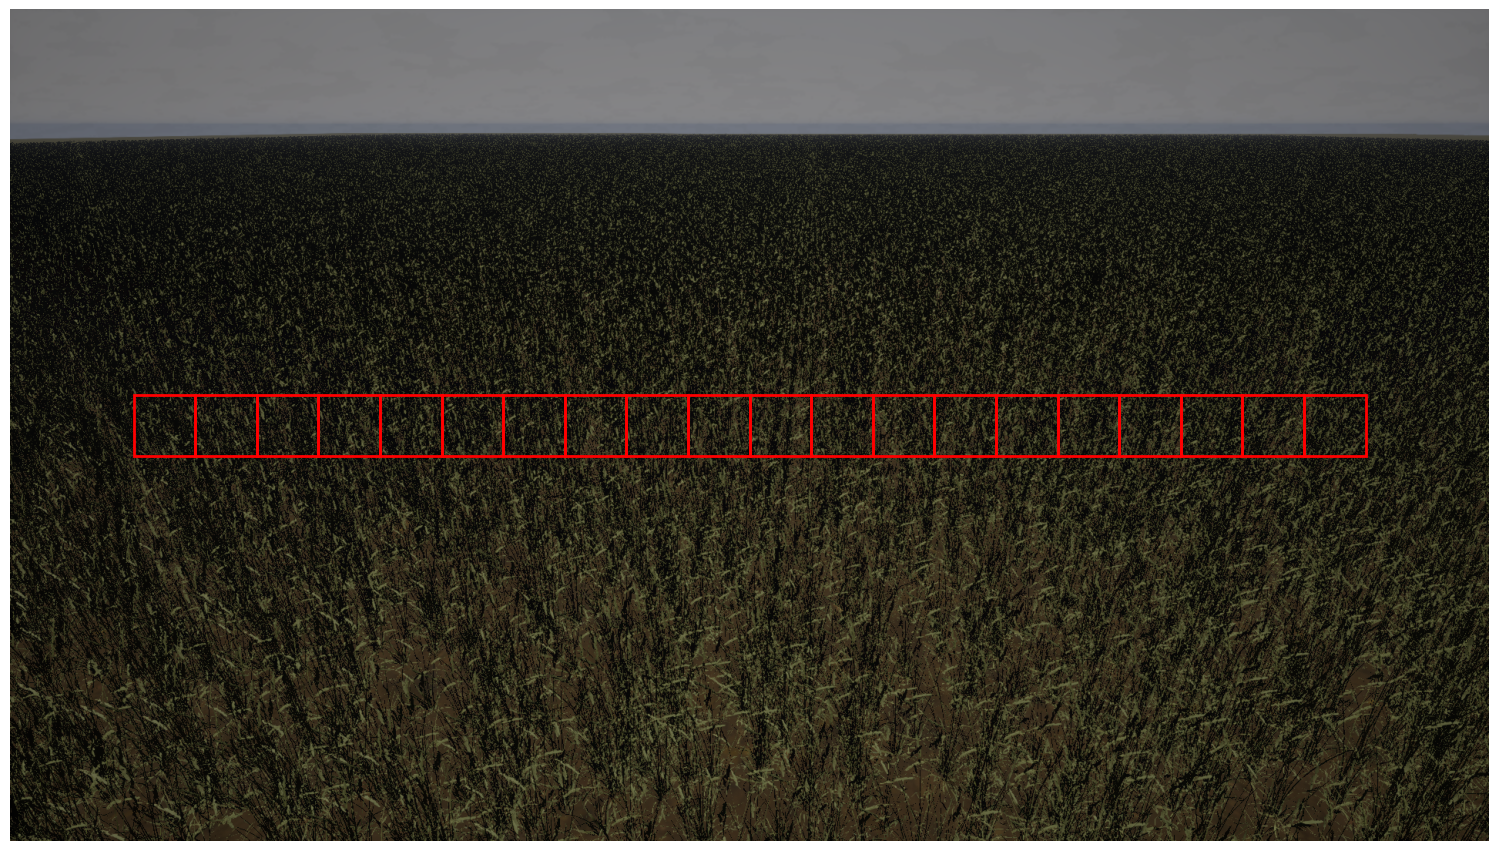
\includegraphics[width=\linewidth]{images/12_img_08GRVI.png}
        \caption{Inherent GRVI = 0.08}
        \label{08}
    \end{subfigure}
    \hfill
    \begin{subfigure}{0.3\textwidth}
        \centering
        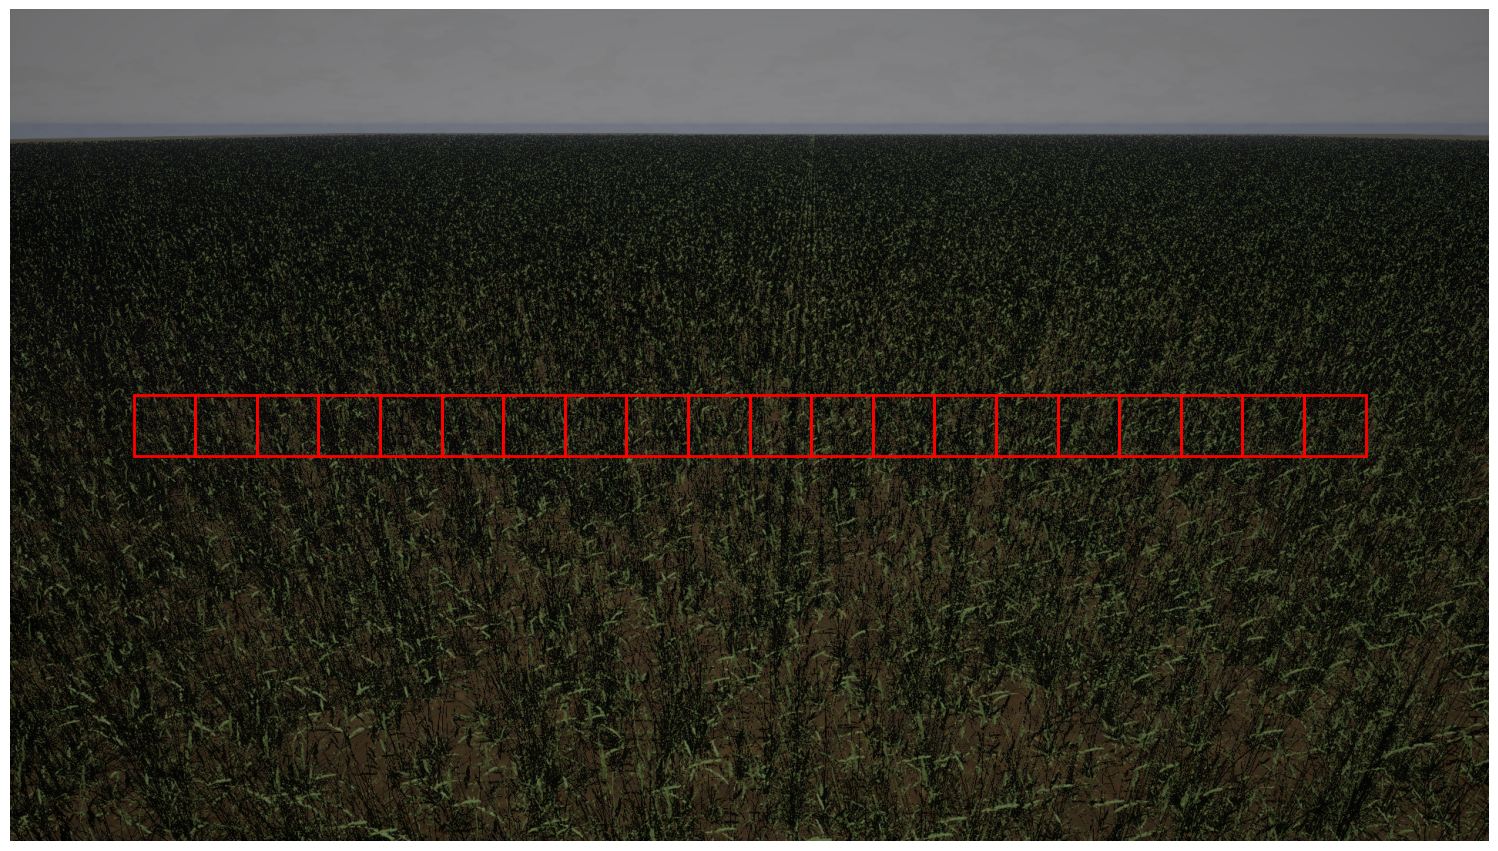
\includegraphics[width=\linewidth]{images/12_img_24GRVI.png}
        \caption{Inherent GRVI = 0.24}
        \label{24}
    \end{subfigure}
    \hfill
    \begin{subfigure}{0.3\textwidth}
        \centering
        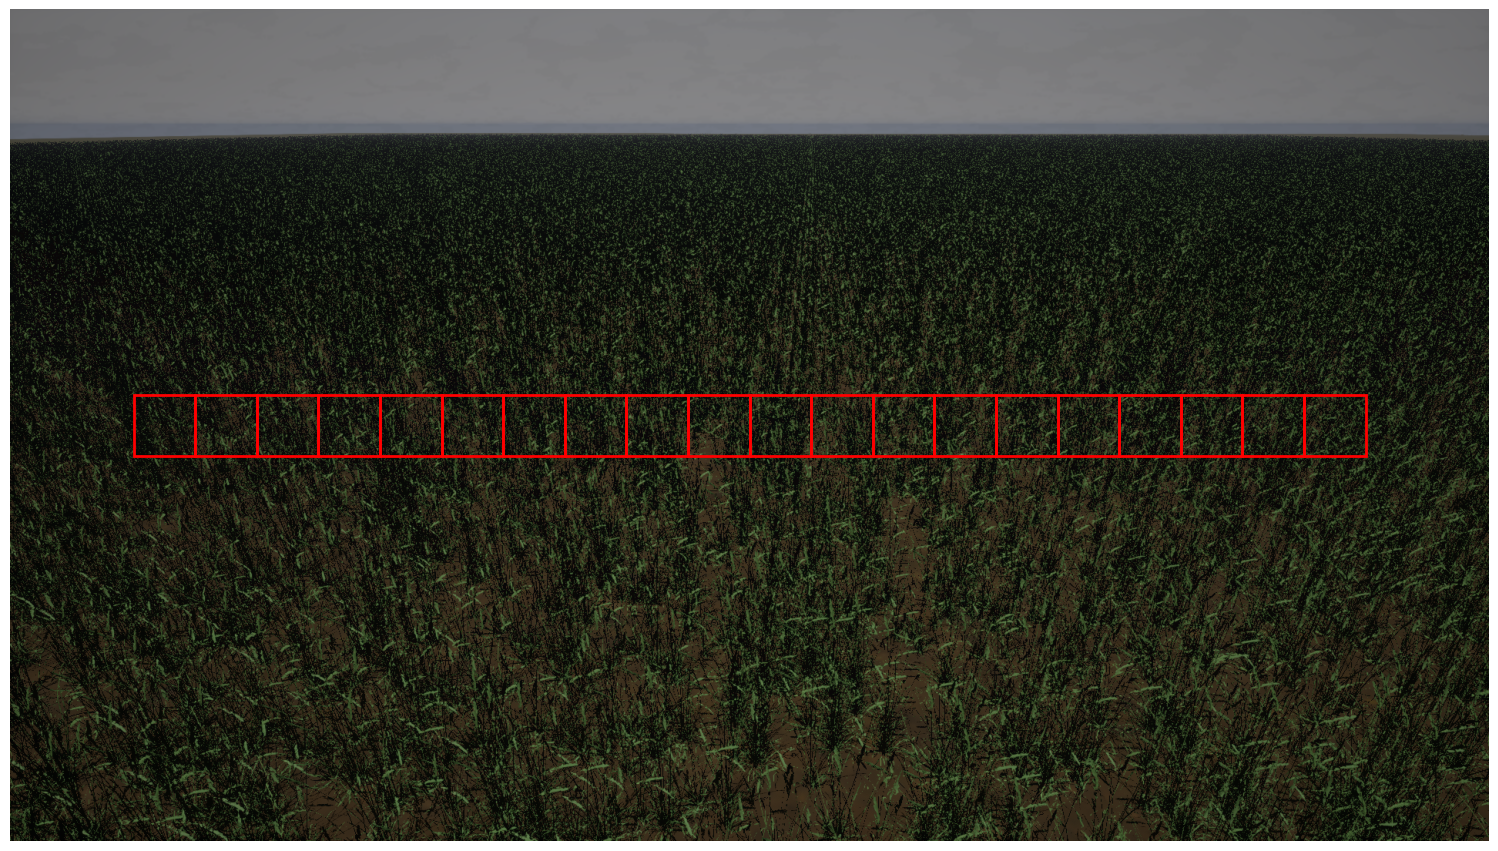
\includegraphics[width=\linewidth]{images/12_img_38GRVI.png}
        \caption{Inherent GRVI = 0.38}
        \label{38}
    \end{subfigure}

    \vspace{0.5cm}

    \begin{subfigure}{0.3\textwidth}
        \centering
        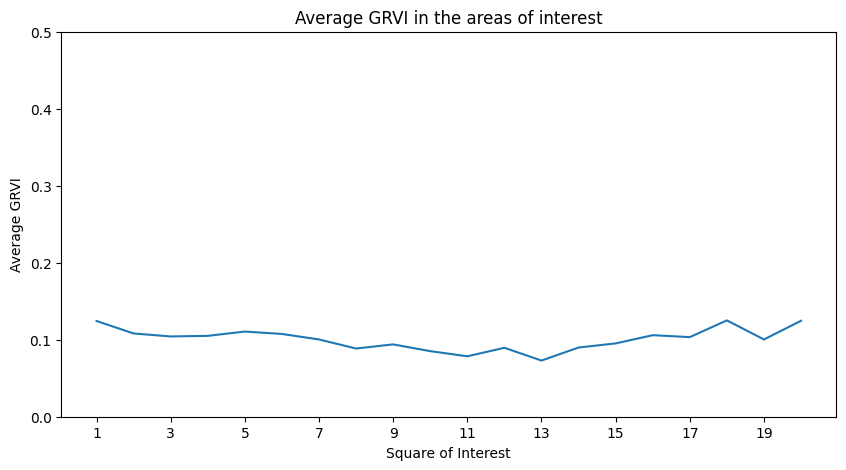
\includegraphics[width=\linewidth]{images/12_graph_08GRVI.png}
        \caption{Inherent GRVI = 0.08}
        \label{08diag}
    \end{subfigure}
    \hfill
    \begin{subfigure}{0.3\textwidth}
        \centering
        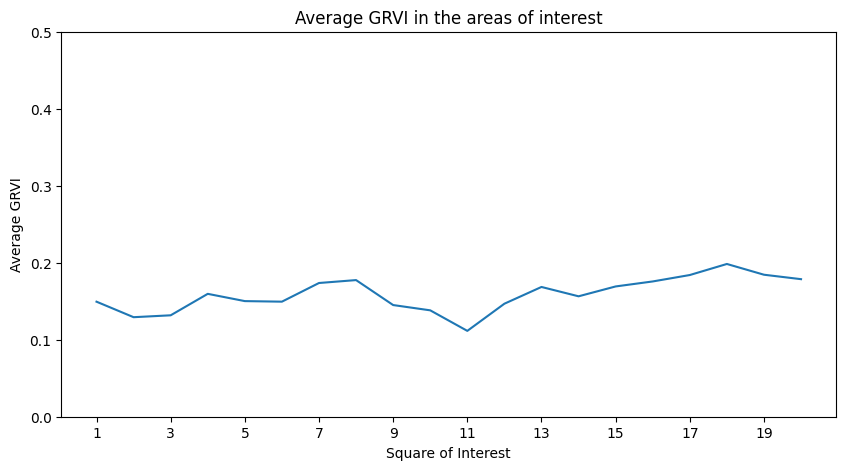
\includegraphics[width=\linewidth]{images/12_graph_24GRVI.png}
        \caption{Inherent GRVI = 0.24}
        \label{24diag}
    \end{subfigure}
    \hfill
    \begin{subfigure}{0.3\textwidth}
        \centering
        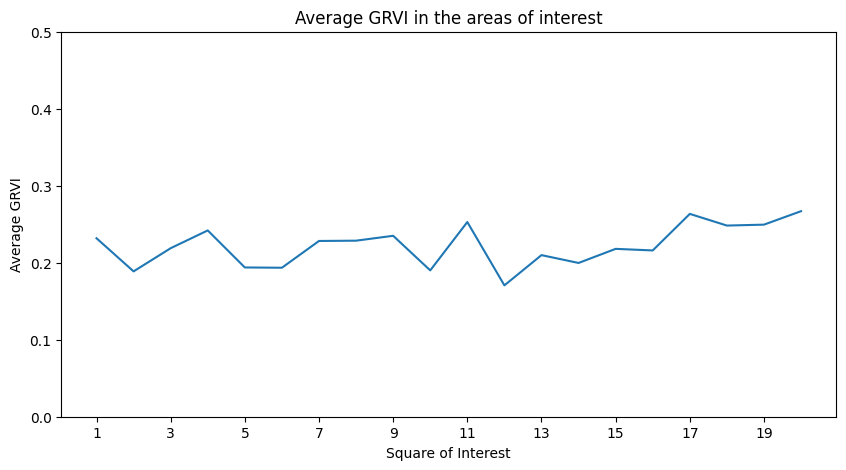
\includegraphics[width=\linewidth]{images/12_graph_38GRVI.png}
        \caption{Inherent GRVI = 0.38}
        \label{38diag}
    \end{subfigure}

    \caption{Images captured under overcast lighting conditions, with SZA fixed at $20^\circ$. The red squares indicate the bounds of the areas-of-interest. The corresponding graphs present the mean calculated GRVI within the individual area-of-interest. The material used for the illustrated plants has an inherent GRVI of 0.08, 0.24 and 0.38, respectively.}
    \label{cloudy-grid}
\end{figure}

The first observation made while reviewing the GRVI per area-of-interest graphs was the susceptibility of different materials to the various sources of error. Particularly, line graphs depicting GRVI values calculated while a high inherent GRVI material is applied appear more jagged, with large dips where planting is not as dense and soil is more visible. On the other hand, line graphs associated with lower GRVI materials appear to be smoother. However, they have a subtle trend towards the frames' edges, implying higher susceptibility to vignetting, caused by lens geometry and light falloff, an effect not as prominent for higher GRVI materials.

Secondly, by reviewing the graphs, a concerning observation regarded the discreteness of different GRVI values, as they are calculated from the collected data. As mentioned before, I have developed $16$ instances of the same material, with their inherent GRVI values ranging from $0.08$ to $0.38$, with a $0.02$ step. As illustrated in Figure~\ref{cloudy-grid}, the range of average GRVI values calculated from data collected under cloudy conditions per material is condensed to $\begin{bmatrix}0.1, & 0.22 \end{bmatrix}$, with the standard deviation of the highest GRVI material for the specific sample being almost $0.029$. That means, that there is potential overlap between different materials' measured GRVI. This motivated me to use all the frames collected during the dummy sequences' executions in order to calculate the average GRVI per material, as that appears in the scene, effectively mapping the inherent value of the material with how it is perceived. The results are presented in Table~\ref{grvi_stats}.


\begin{table}[htb]
    \centering
    \caption{Calculated mean GRVI and standard deviation for different inherent GRVI values.}
    \label{grvi_stats}
    \renewcommand{\arraystretch}{1.15}
    \begin{tabular}{c!{\vrule width 1.2pt}cc}
        \hline
        \textbf{Inherent GRVI} & \textbf{Calculated mean GRVI} & \textbf{Standard deviation} \\
        \hline
        \textbf{0.08} & 0.10066 & 0.01408 \\
        \textbf{0.10} & 0.10659 & 0.01422 \\
        \textbf{0.12} & 0.11679 & 0.01303 \\
        \textbf{0.14} & 0.12733 & 0.01587 \\
        \textbf{0.16} & 0.12052 & 0.01520 \\
        \textbf{0.18} & 0.12764 & 0.02197 \\
        \textbf{0.20} & 0.13732 & 0.02435 \\
        \textbf{0.22} & 0.13737 & 0.01772 \\
        \textbf{0.24} & 0.15887 & 0.02141 \\
        \textbf{0.26} & 0.16545 & 0.01875 \\
        \textbf{0.28} & 0.17287 & 0.02794 \\
        \textbf{0.30} & 0.18425 & 0.01657 \\
        \textbf{0.32} & 0.19349 & 0.02847 \\
        \textbf{0.34} & 0.19938 & 0.03181 \\
        \textbf{0.36} & 0.21248 & 0.02474 \\
        \textbf{0.38} & 0.22228 & 0.02641 \\
        \hline
    \end{tabular}
\end{table}

Table~\ref{grvi_stats} validates the previously expressed concerns. Although every inherent GRVI value maps to a calculated mean value, and both sides follow an upward trend - with the only outlier being the inherent value $0.16$, whose associated calculated value is lower than the one associated with the inherent value $0.14$ - the standard deviation of the calculations is relatively high, causing overlapping perceived GRVI values between different inherent values. It is also validated that the standard deviation tends to be higher for materials with relatively high inherent GRVI. 

As mentioned in the beginning of the \hyperref[datasssessment]{Data Assessment} section, dummy render sequences have been performed while a higher planting density was applied to the simulated field. For the assessment of the target values, it was important that I perform the same tests for the materials, as they appear during data collection. To achieve this, I identified which part of the field is depicted in every captured frame using the camera location data. For each frame, I calculated the average GRVI value of all the areas-of-interest depicting the same parts of the field, considering that in many captured frames, more than one parts are included, each with different applied wheat material, along with the standard deviation. Finally, I calculated the mean of the each previously calculated average that corresponds to parts of the field with the same material applied, along with the mean standard deviation.

The results are presented in Table~\ref{grvi_stats_ld}. It can be seen that the more prominent appearance of soil made the calculated GRVI to be reduced to less than half of the values tracked during the dummy renders, compressing the values even further to the $\begin{bmatrix}0.03865, & 0.11580\end{bmatrix}$ range, again, with relatively high standard deviation. However, their structure is still reasonable, with the perceived GRVI averages increasing as the corresponding assigned GRVI increases for almost all the cases.  

\begin{table}[htb]
    \centering
    \caption{Calculated mean GRVI and standard deviation for different inherent GRVI values.}
    \label{grvi_stats_ld}
    \renewcommand{\arraystretch}{1.15}
    \begin{tabular}{c!{\vrule width 1.2pt}cc}
        \hline
        \textbf{Inherent GRVI} & \textbf{Calculated mean GRVI} & \textbf{Standard deviation} \\
        \hline
        \textbf{0.08} & 0.03865 & 0.01138 \\
        \textbf{0.10} & 0.05840 & 0.01201 \\
        \textbf{0.12} & 0.05827 & 0.01102 \\
        \textbf{0.14} & 0.06596 & 0.01216 \\
        \textbf{0.16} & 0.06829 & 0.00959 \\
        \textbf{0.18} & 0.07512 & 0.01113 \\
        \textbf{0.20} & 0.08219 & 0.01363 \\
        \textbf{0.22} & 0.08231 & 0.01534 \\
        \textbf{0.24} & 0.08663 & 0.01367 \\
        \textbf{0.26} & 0.09405 & 0.01426 \\
        \textbf{0.28} & 0.10152 & 0.01515 \\
        \textbf{0.30} & 0.09916 & 0.01549 \\
        \textbf{0.32} & 0.10949 & 0.01665 \\
        \textbf{0.34} & 0.11360 & 0.01665 \\
        \textbf{0.36} & 0.11525 & 0.01743 \\
        \textbf{0.38} & 0.11580 & 0.01866 \\
        \hline
    \end{tabular}
\end{table}

Both in the cases of dummy and final renders, the calculated means of GRVI show the general behavior of the perceived GRVI, as the applied material instance changes. As mentioned before though, the fluctuations of the perceived values, hinted through the standard deviation, are averaged out. These fluctuations prevent us from simply mapping the average perceived values to the assigned GRVI of each material, due to the value overlaps they cause. To understand better the degree of overlap between the perceived values that correspond to different inherent values, I constructed a perceived GRVI map, where each presented value is the average perceived GRVI value for the corresponding part of the field. This map was the compared to the map of the field that presents the inherent GRVI values. The two maps are illustrated in Figure~\ref{grvi-maps}. 

\begin{figure}[htb]
    \centering
    
    \begin{subfigure}{0.48\linewidth}
        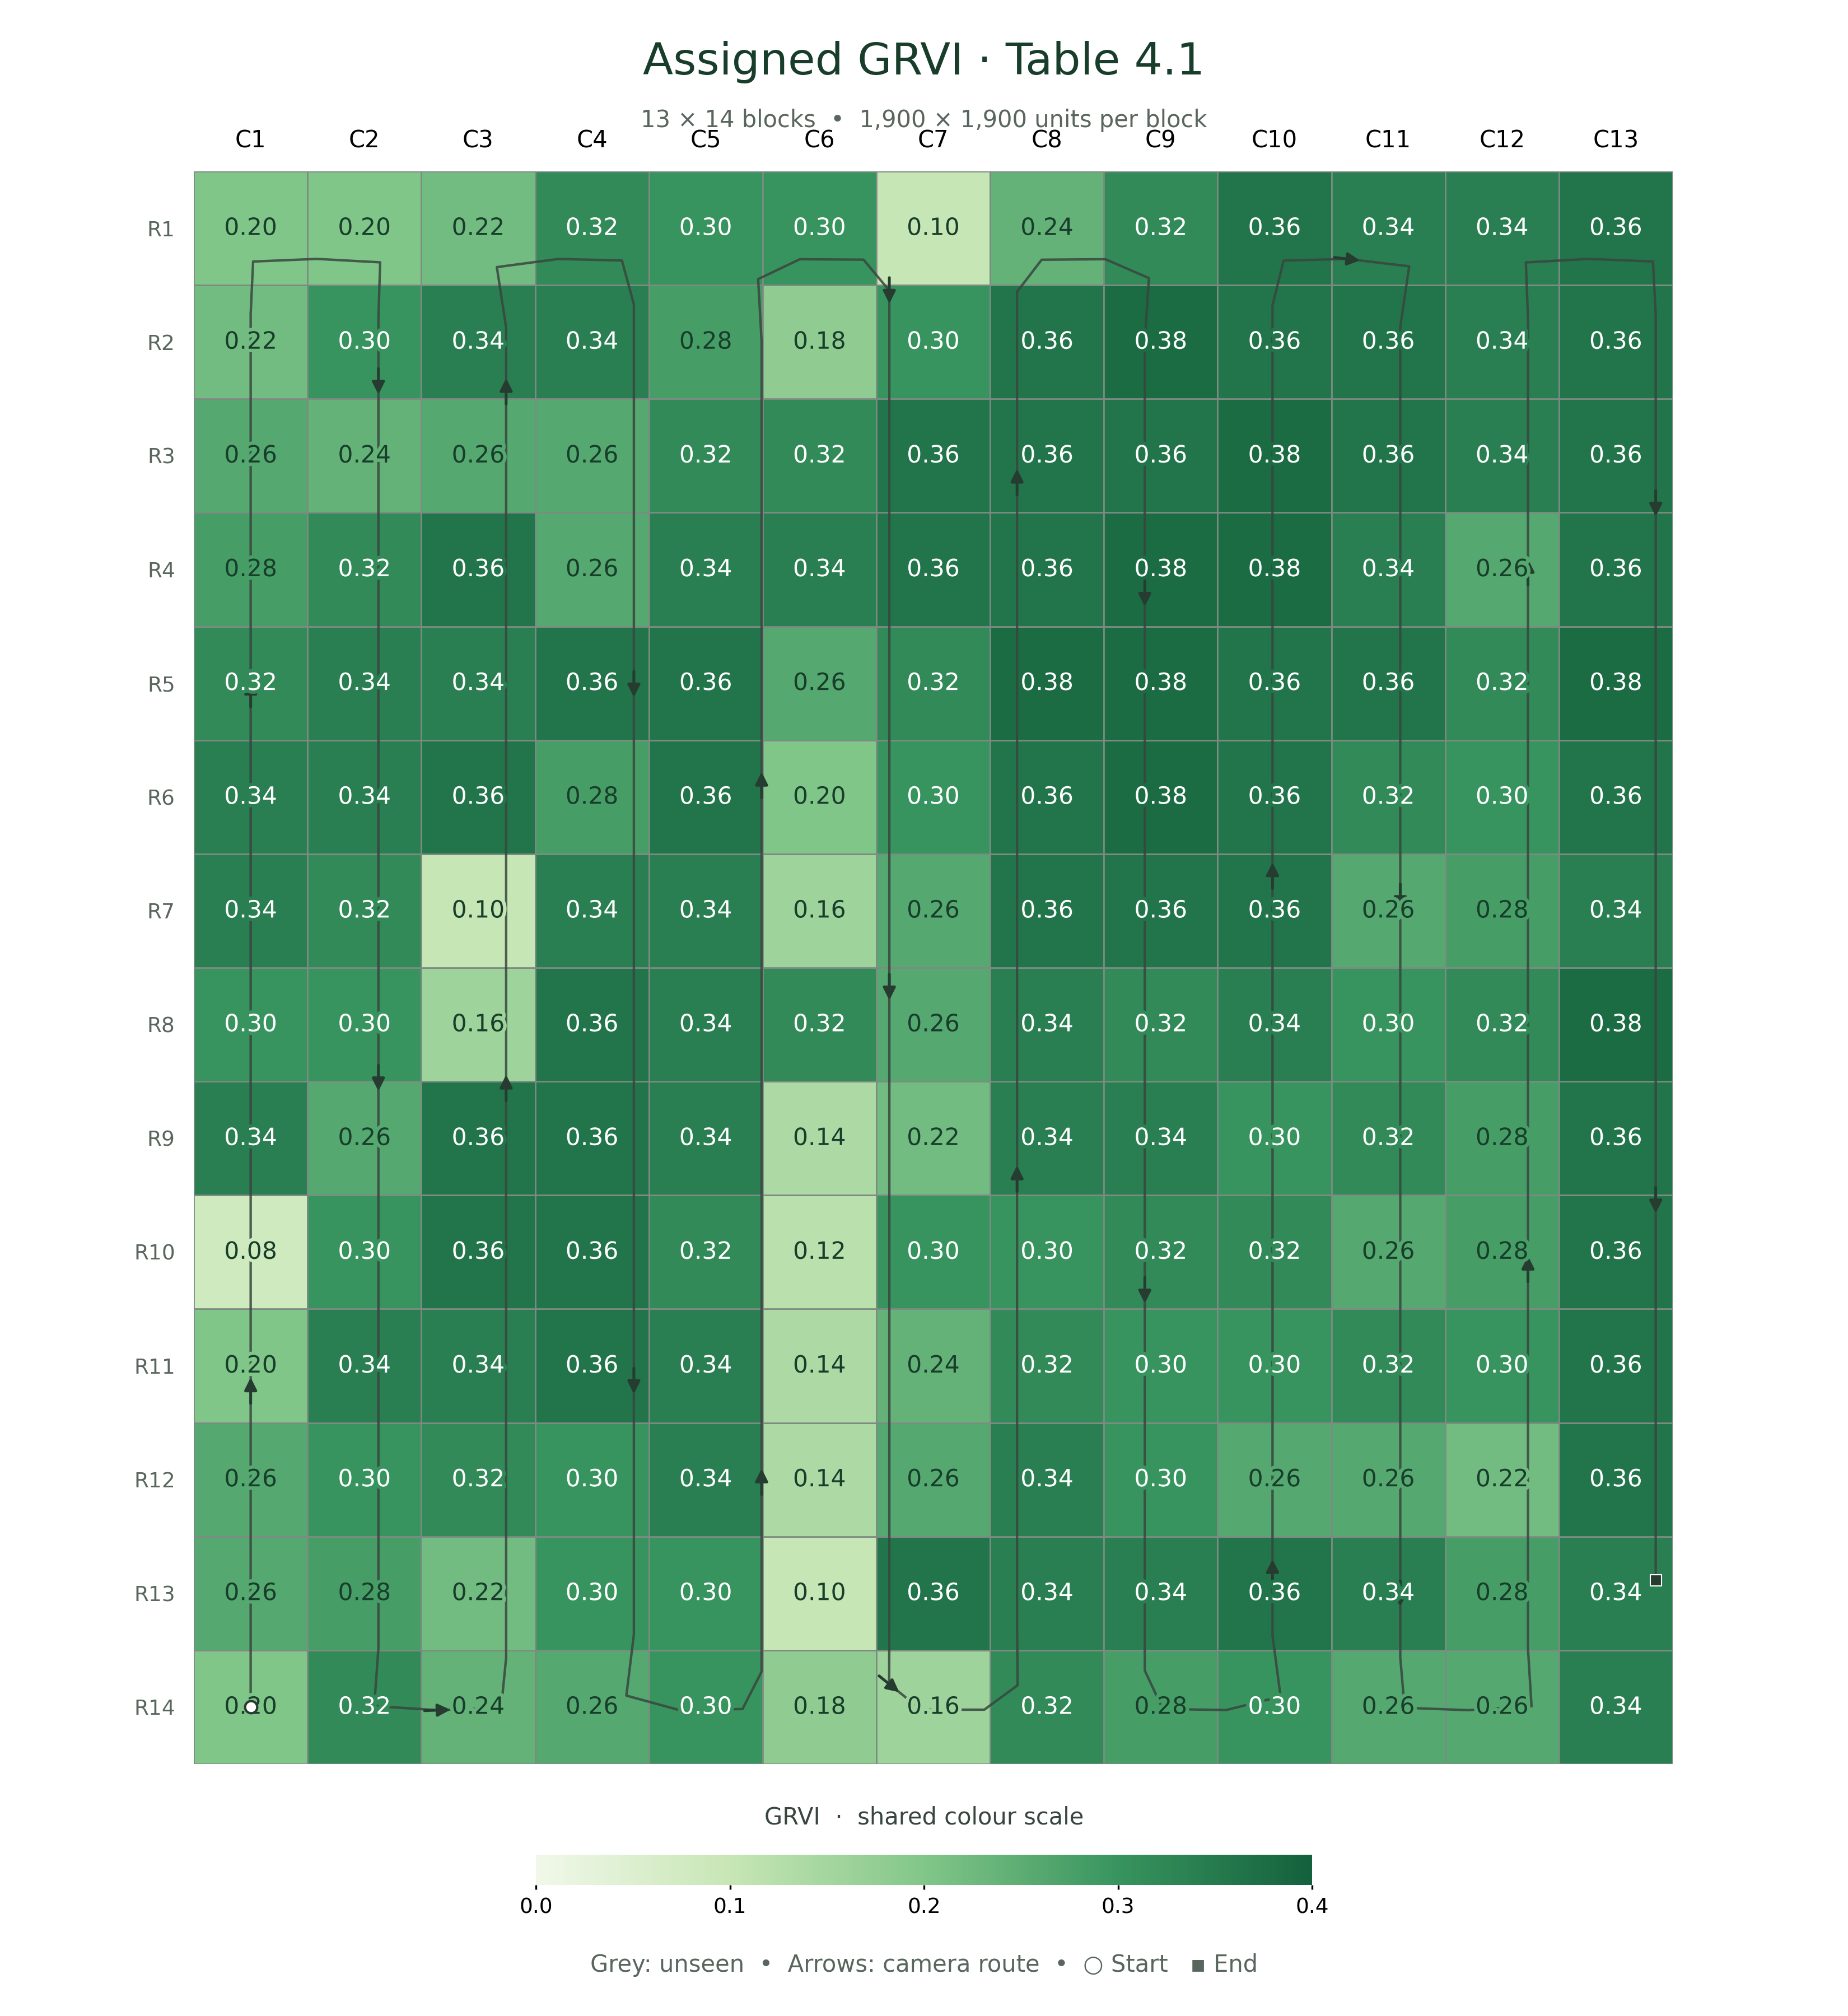
\includegraphics[width=\linewidth]{images/assigned_grvi_map.png}
        \caption{Map of assigned GRVI values per part of the field.}
        \label{assigned-map}
    \end{subfigure}\hfill
    \begin{subfigure}{0.48\linewidth}
        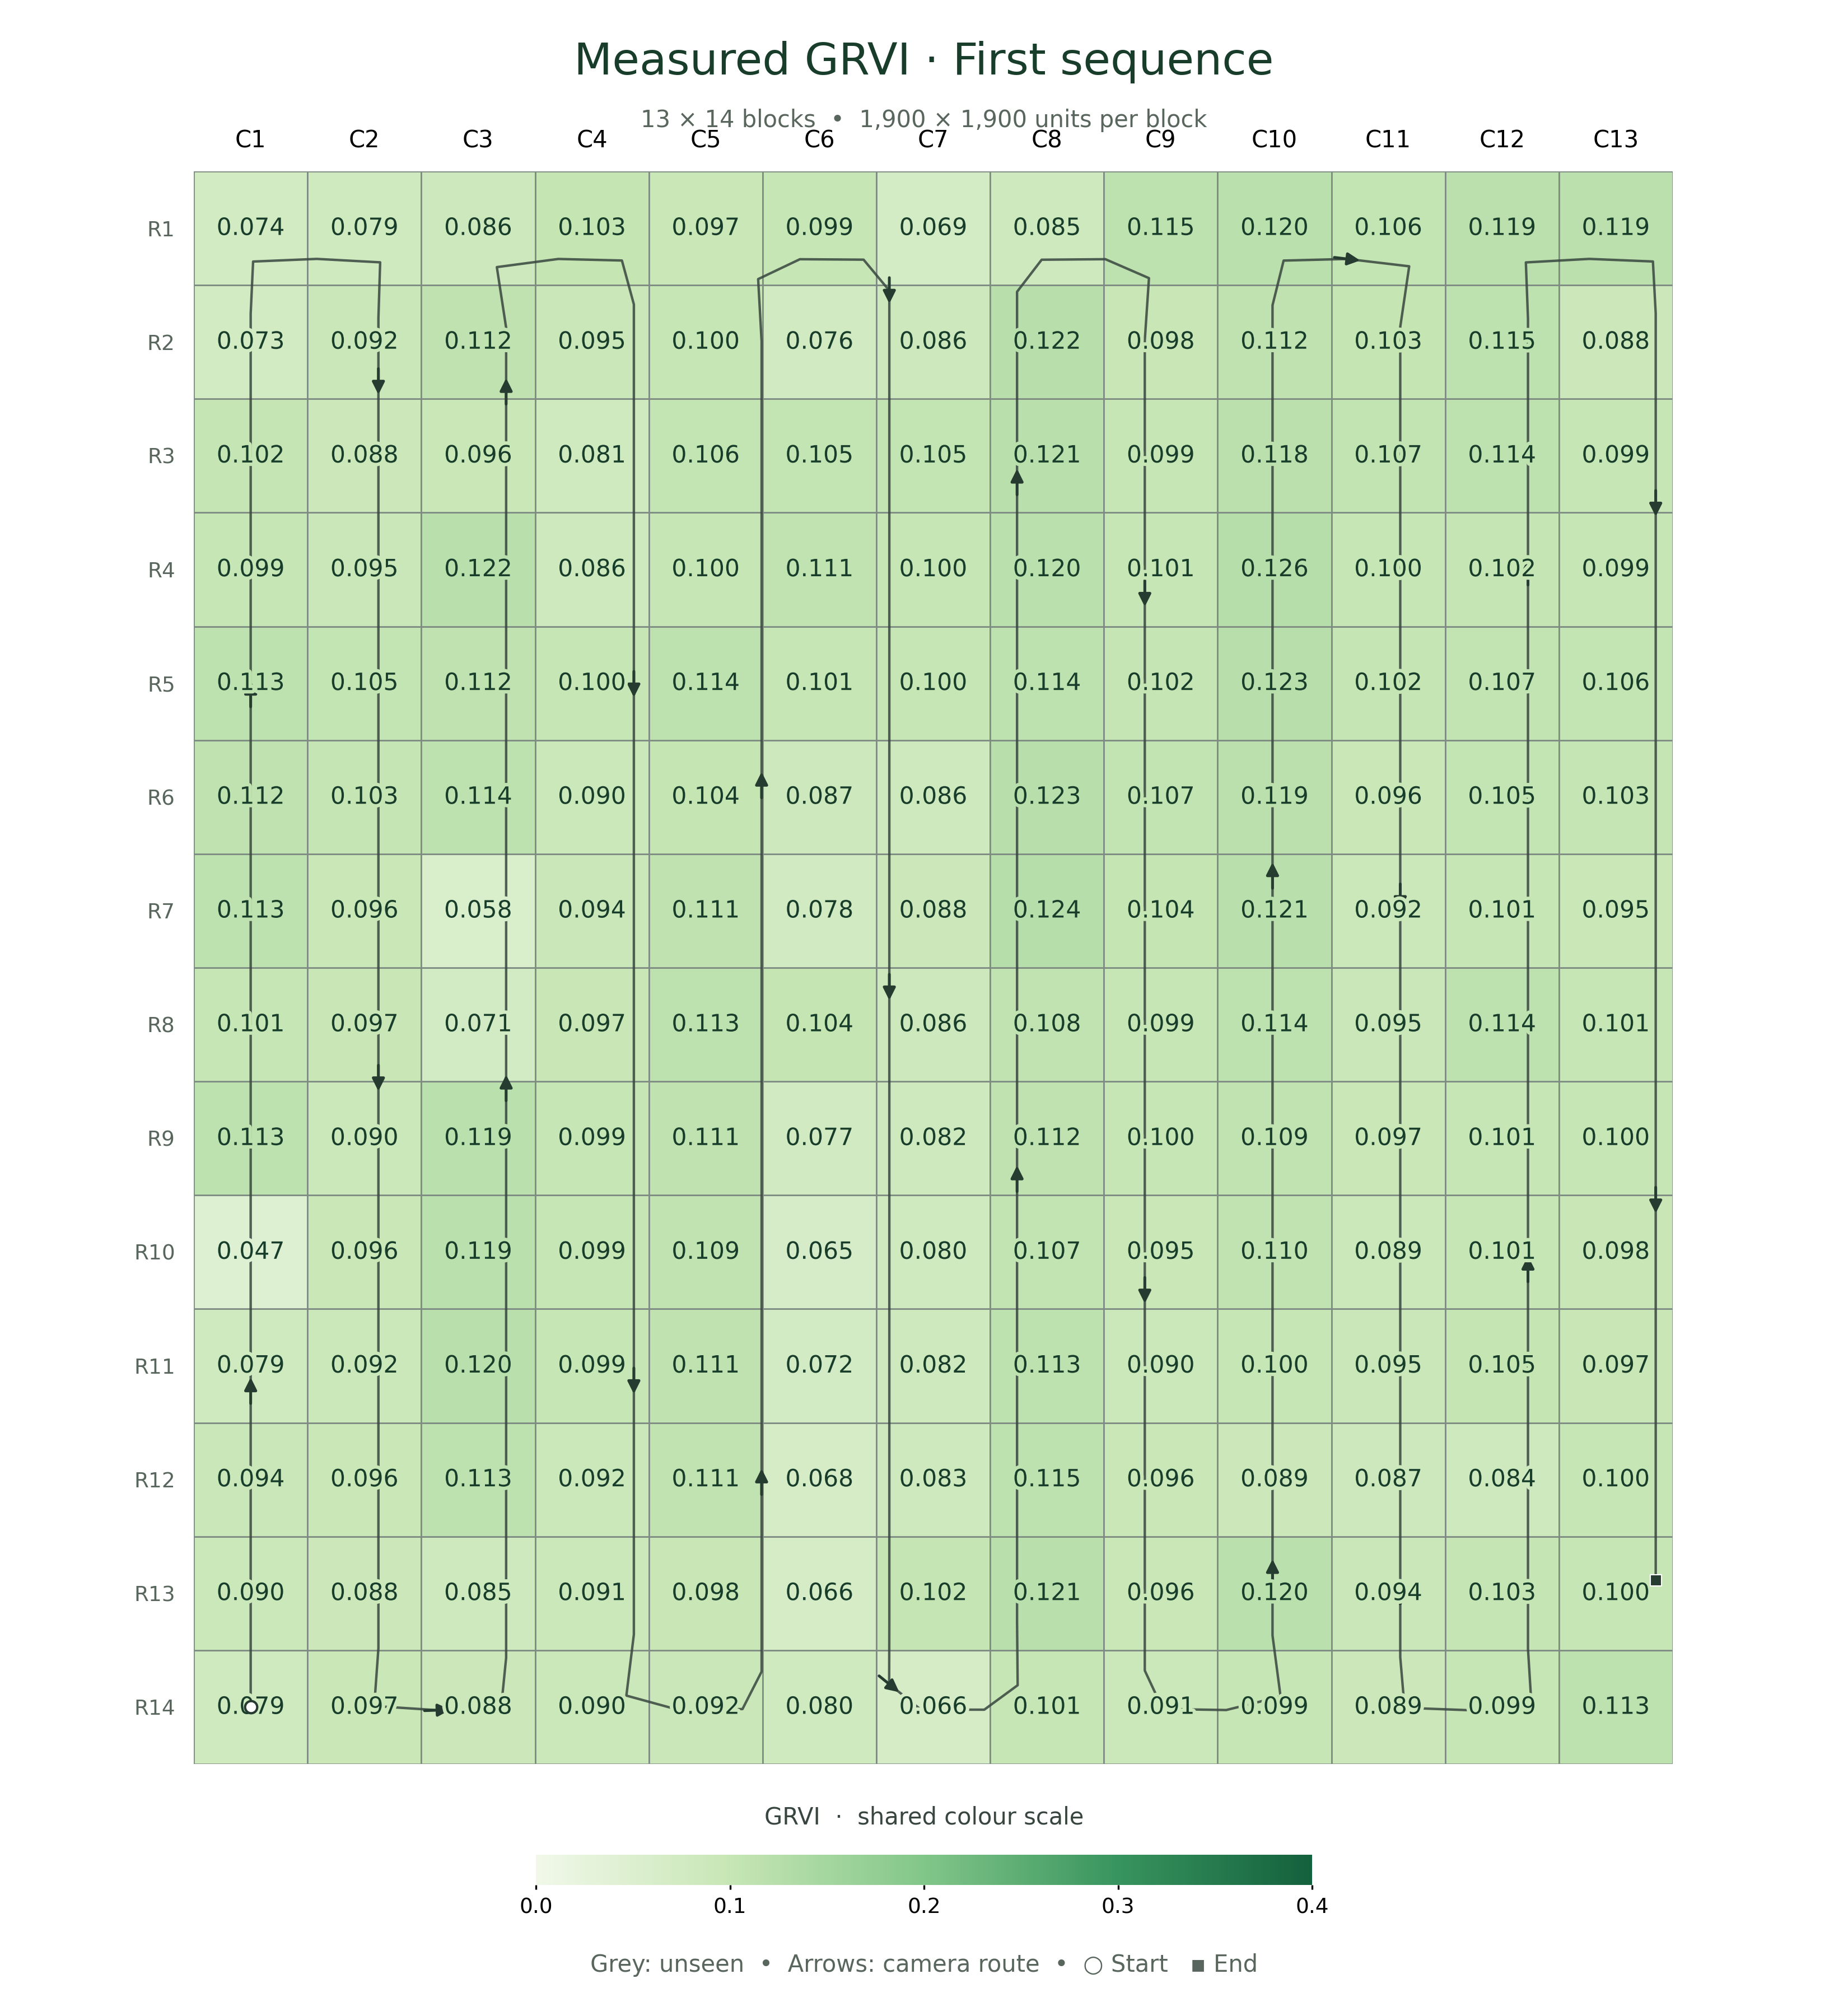
\includegraphics[width=\linewidth]{images/measured_grvi_map.png}
        \caption{Map of measured GRVI values per part of the field.}
        \label{measured-map}
    \end{subfigure}
    
    \caption{Both assigned and measured GRVI maps of the field. The arrows indicate the path the camera follows during data collection.}
    \label{grvi-maps}
\end{figure}

With multiple multiple cases of overlapping measured GRVI values between parts of the field with different materials assigned, I doubted whether using these values in their raw form is meaningful. An application that also accounts for factors other than the reflectance of the plants' surface could benefit from them. On any other case, using either directly the assigned GRVI or the measured GRVI averages, whichever achieves higher predictive performance, should be more beneficial.

In parallel with the investigation of the degree of overlap, I performed clustering on the measured values. The objective was to uncover whether it is reasonable to expect the measured values to be divided into $16$ groups, as many as the developed material instances. Specifically, as a first step, I re-used the average perceived GRVI of the areas-of-interest in each captured frame, previously calculated in order to construct the map illustrated in Figure~\ref{measured-map}. Next, I performed K-Means clustering using the calculated averages as inputs. All numbers of clusters between $2$ and $16$ were tested. Several of the results are illustrated in Figure~\ref{kmeans}.

\begin{figure} [htb]
    \centering
    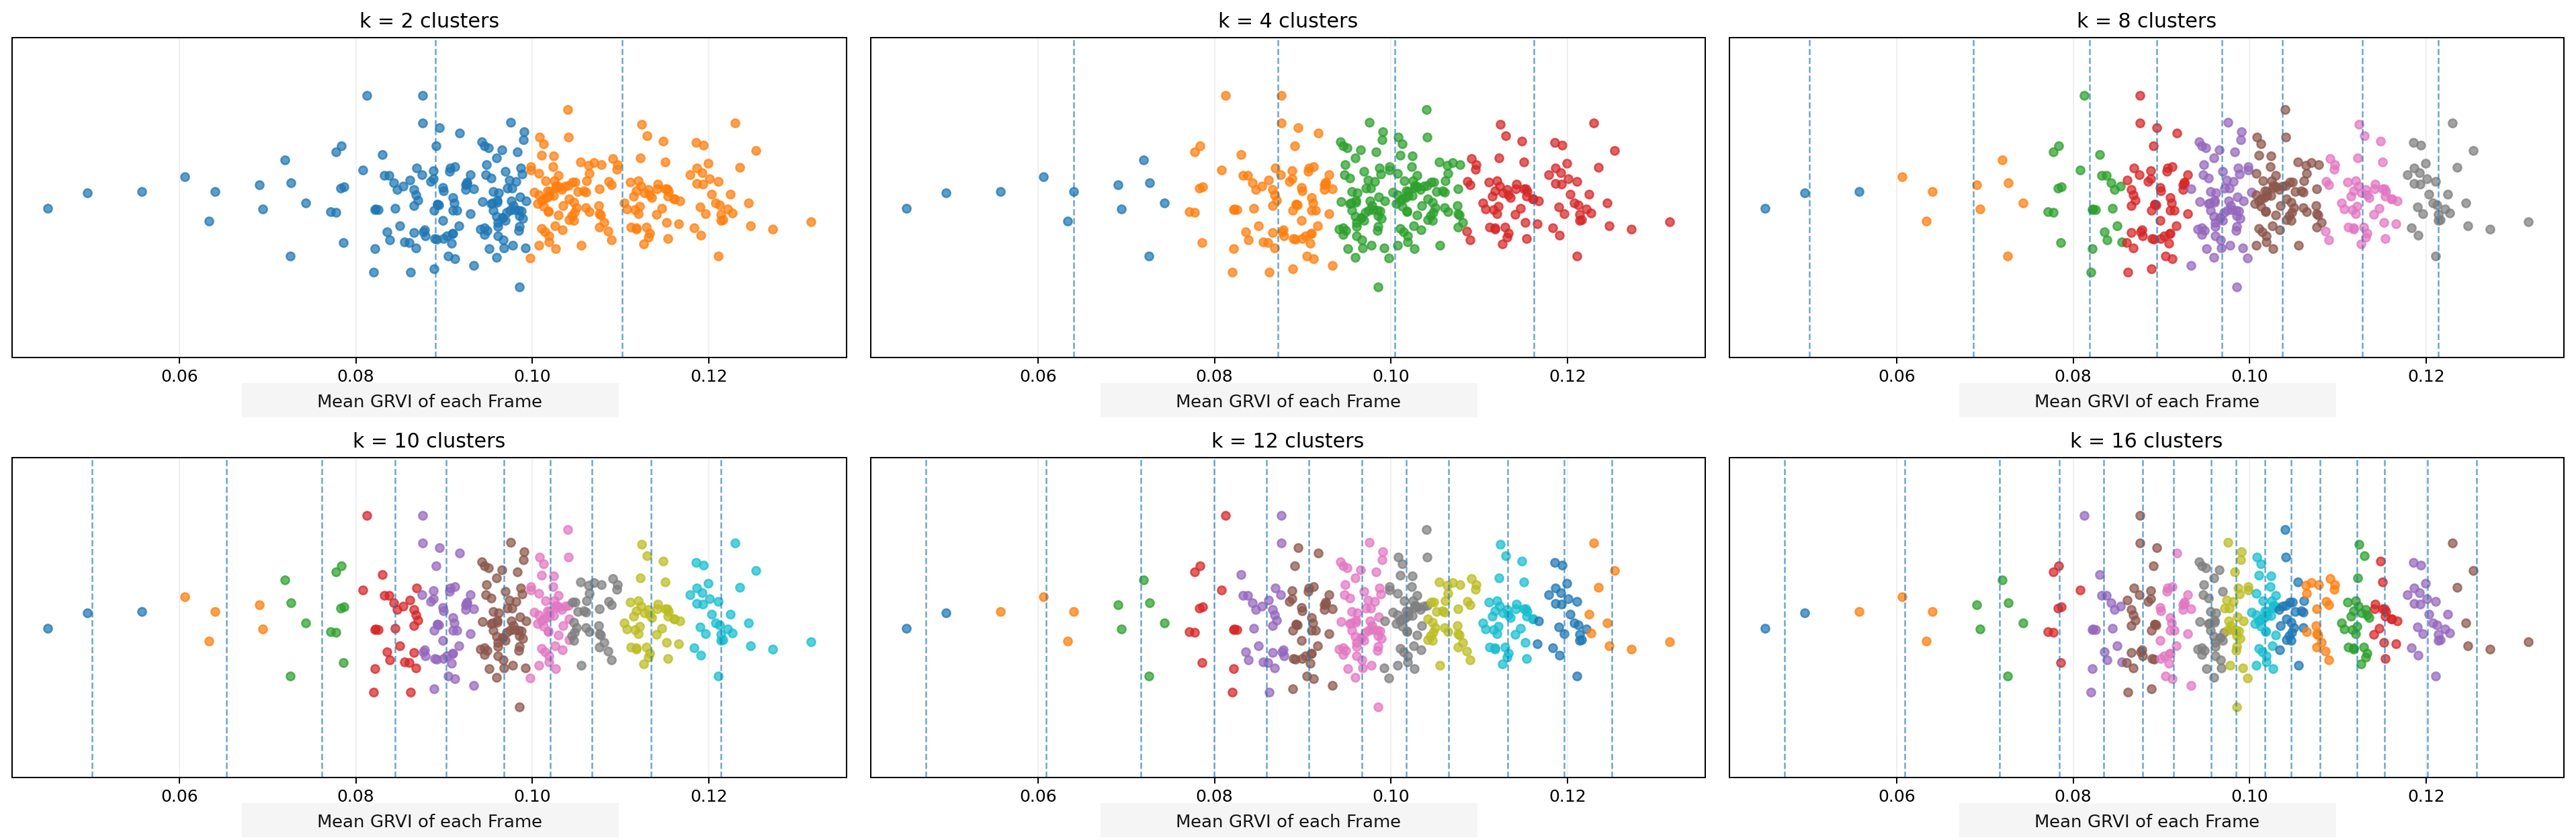
\includegraphics[width=1\linewidth]{images/cloudy-clusters.png}
    \caption{K-Means clustering performed with the average GRVI per frame as inputs, for different amounts of clusters. Random vertical offset was applied to the different points for clearer demonstration.}
    \label{kmeans}
\end{figure}

Using silhouette score as the primary evaluation metric, the results for different amounts of clusters were relatively close. Specifically, a silhouette score higher than $0.53$ was achieved for all the amounts of clusters tested, with the highest score being $0.562$ for four clusters. For $16$ clusters, being the ideal amount since it matches the amount of materials, the achieved score was $0.542$. Although $16$ clusters did not provide a separation as coarse as $4$, it was still considered as a viable option, due to the minimal loss of clustering quality. 

\subsection{GRVI Affected by Shadows}
\label{shadows-aff-grvi}


Shadows are also expected to affect the calculations of the perceived GRVI values. I found it therefore necessary to investigate the degree at which this occurs, examining whether it is actually meaningful to include shadows to the error factors the proposed models aim to address. All the tests were performed using data collected during the final render sequences.

The first conducted experiment aimed to check how the GRVI of different materials is perceived in shaded parts of the field. Having performed data data collection beforehand, I selected the samples captured while the absolute value of SZA was set to $85^\circ$ and calculated the average perceived GRVI per different material. I chose to use the absolute value rather than either the positive or negative, since in both cases, green- and red-band illuminance is the same but, the areas that are shaded in one case are not shaded in the other. That means that, if only one SZA was selected, some materials would not appear shaded, and metrics would not be extracted. 

The results are presented in Table~\ref{grvi_stats_gloomy}. Despite the expected upward trend of the calculated means as the assigned values increase, there were several concerning observations. For starters, the standard deviation is particularly high, indicating a high degree of variance between the samples. The monotonicity is also interrupted in more points compared to the values presented in the diffuse lighting section. Finally, this is the first case in which negative GRVI values are observed. 


\begin{table}[htb]
    \centering
    \caption{Calculated mean GRVI and standard deviation for different inherent GRVI values for frames depicting shaded scenes. SZA was set to $\pm 85^\circ$.}
    \label{grvi_stats_gloomy}
    \renewcommand{\arraystretch}{1.15}
    \begin{tabular}{c!{\vrule width 1.2pt}cc}
        \hline
        \textbf{Inherent GRVI} & \textbf{Calculated mean GRVI} & \textbf{Standard deviation} \\
        \hline
        \textbf{0.08} & -0.07121 & 0.06419 \\
        \textbf{0.10} & -0.01105 & 0.16058 \\
        \textbf{0.12} & -0.00470 & 0.07888 \\
        \textbf{0.14} & 0.02134 & 0.09981 \\
        \textbf{0.16} & 0.04428 & 0.08928 \\
        \textbf{0.18} & -0.13216 & 0.07311 \\
        \textbf{0.20} & 0.01871 & 0.09108 \\
        \textbf{0.22} & 0.05434 & 0.09088 \\
        \textbf{0.24} & 0.06008 & 0.10230 \\
        \textbf{0.26} & 0.07818 & 0.07561 \\
        \textbf{0.28} & 0.06839 & 0.08143 \\
        \textbf{0.30} & 0.07080 & 0.08523 \\
        \textbf{0.32} & 0.10111 & 0.07727 \\
        \textbf{0.34} & 0.09300 & 0.07372 \\
        \textbf{0.36} & 0.11045 & 0.07813 \\
        \textbf{0.38} & 0.11496 & 0.07893 \\
        \hline
    \end{tabular}
\end{table}


Further inspection of both the raw frames and the extracted data helped with the identification of multiple contributing factors for the existence of both negative values and high degree of variance. These factors were introduced with the inclusion of shadows in the scene and were exceptionally difficult to address, since some of them are uncontrollable to a degree, while others require solutions that will harm the consistency of the dataset. One of them is the shadow's consistency, considering that the cast shadow is not the result of a solid material but rather is cast by the leaves and branches of the tree mesh, leaving bright spots or incomplete light blockage at several points. The presence of sources other than Directional Light also plays an important role. Since Directional Light is cut off, these parts of the field are illuminated by other mechanisms, including the Sky Light actor and Lumen, whose red-green balance is different than the Directional Light's, affecting the red and green illuminance values measured by the light meters. Other suspected factors are the presence of soil, sensor artifacts caused by low lighting and disproportionate changes between the illuminance values for each band and luminance values for each band.

It was unclear wether these factors affect the dataset as a whole or just create large amounts of outliers, harming the calculated mean values. In order to clarify this, I performed the Median Absolute Deviation (MAD) method in order to identify and exclude possible outliers. That said, even after excluding the detected outliers, there was no noticeable change in the calculated means.

It was also tested whether different SZA values affect the measured GRVI for a shaded area. Specifically, I randomly selected frames depicting shaded parts of the field, each having materials with different inherent GRVI values, and compared the average GRVI values measured within them with the averages calculated using frames of the same parts of the scene but with different set SZA values - naturally, for SZA values where the examined parts remain shaded. The measured values for three of the selected materials are illustrated in Figure~\ref{gloomy-diff-mats-and-sza}. It can be seen that the perceived GRVI of materials with high inherent GRVI increases as the absolute value of SZA increases, while the opposite happens for materials with low inherent GRVI. 


\begin{figure} [htb]
    \centering
    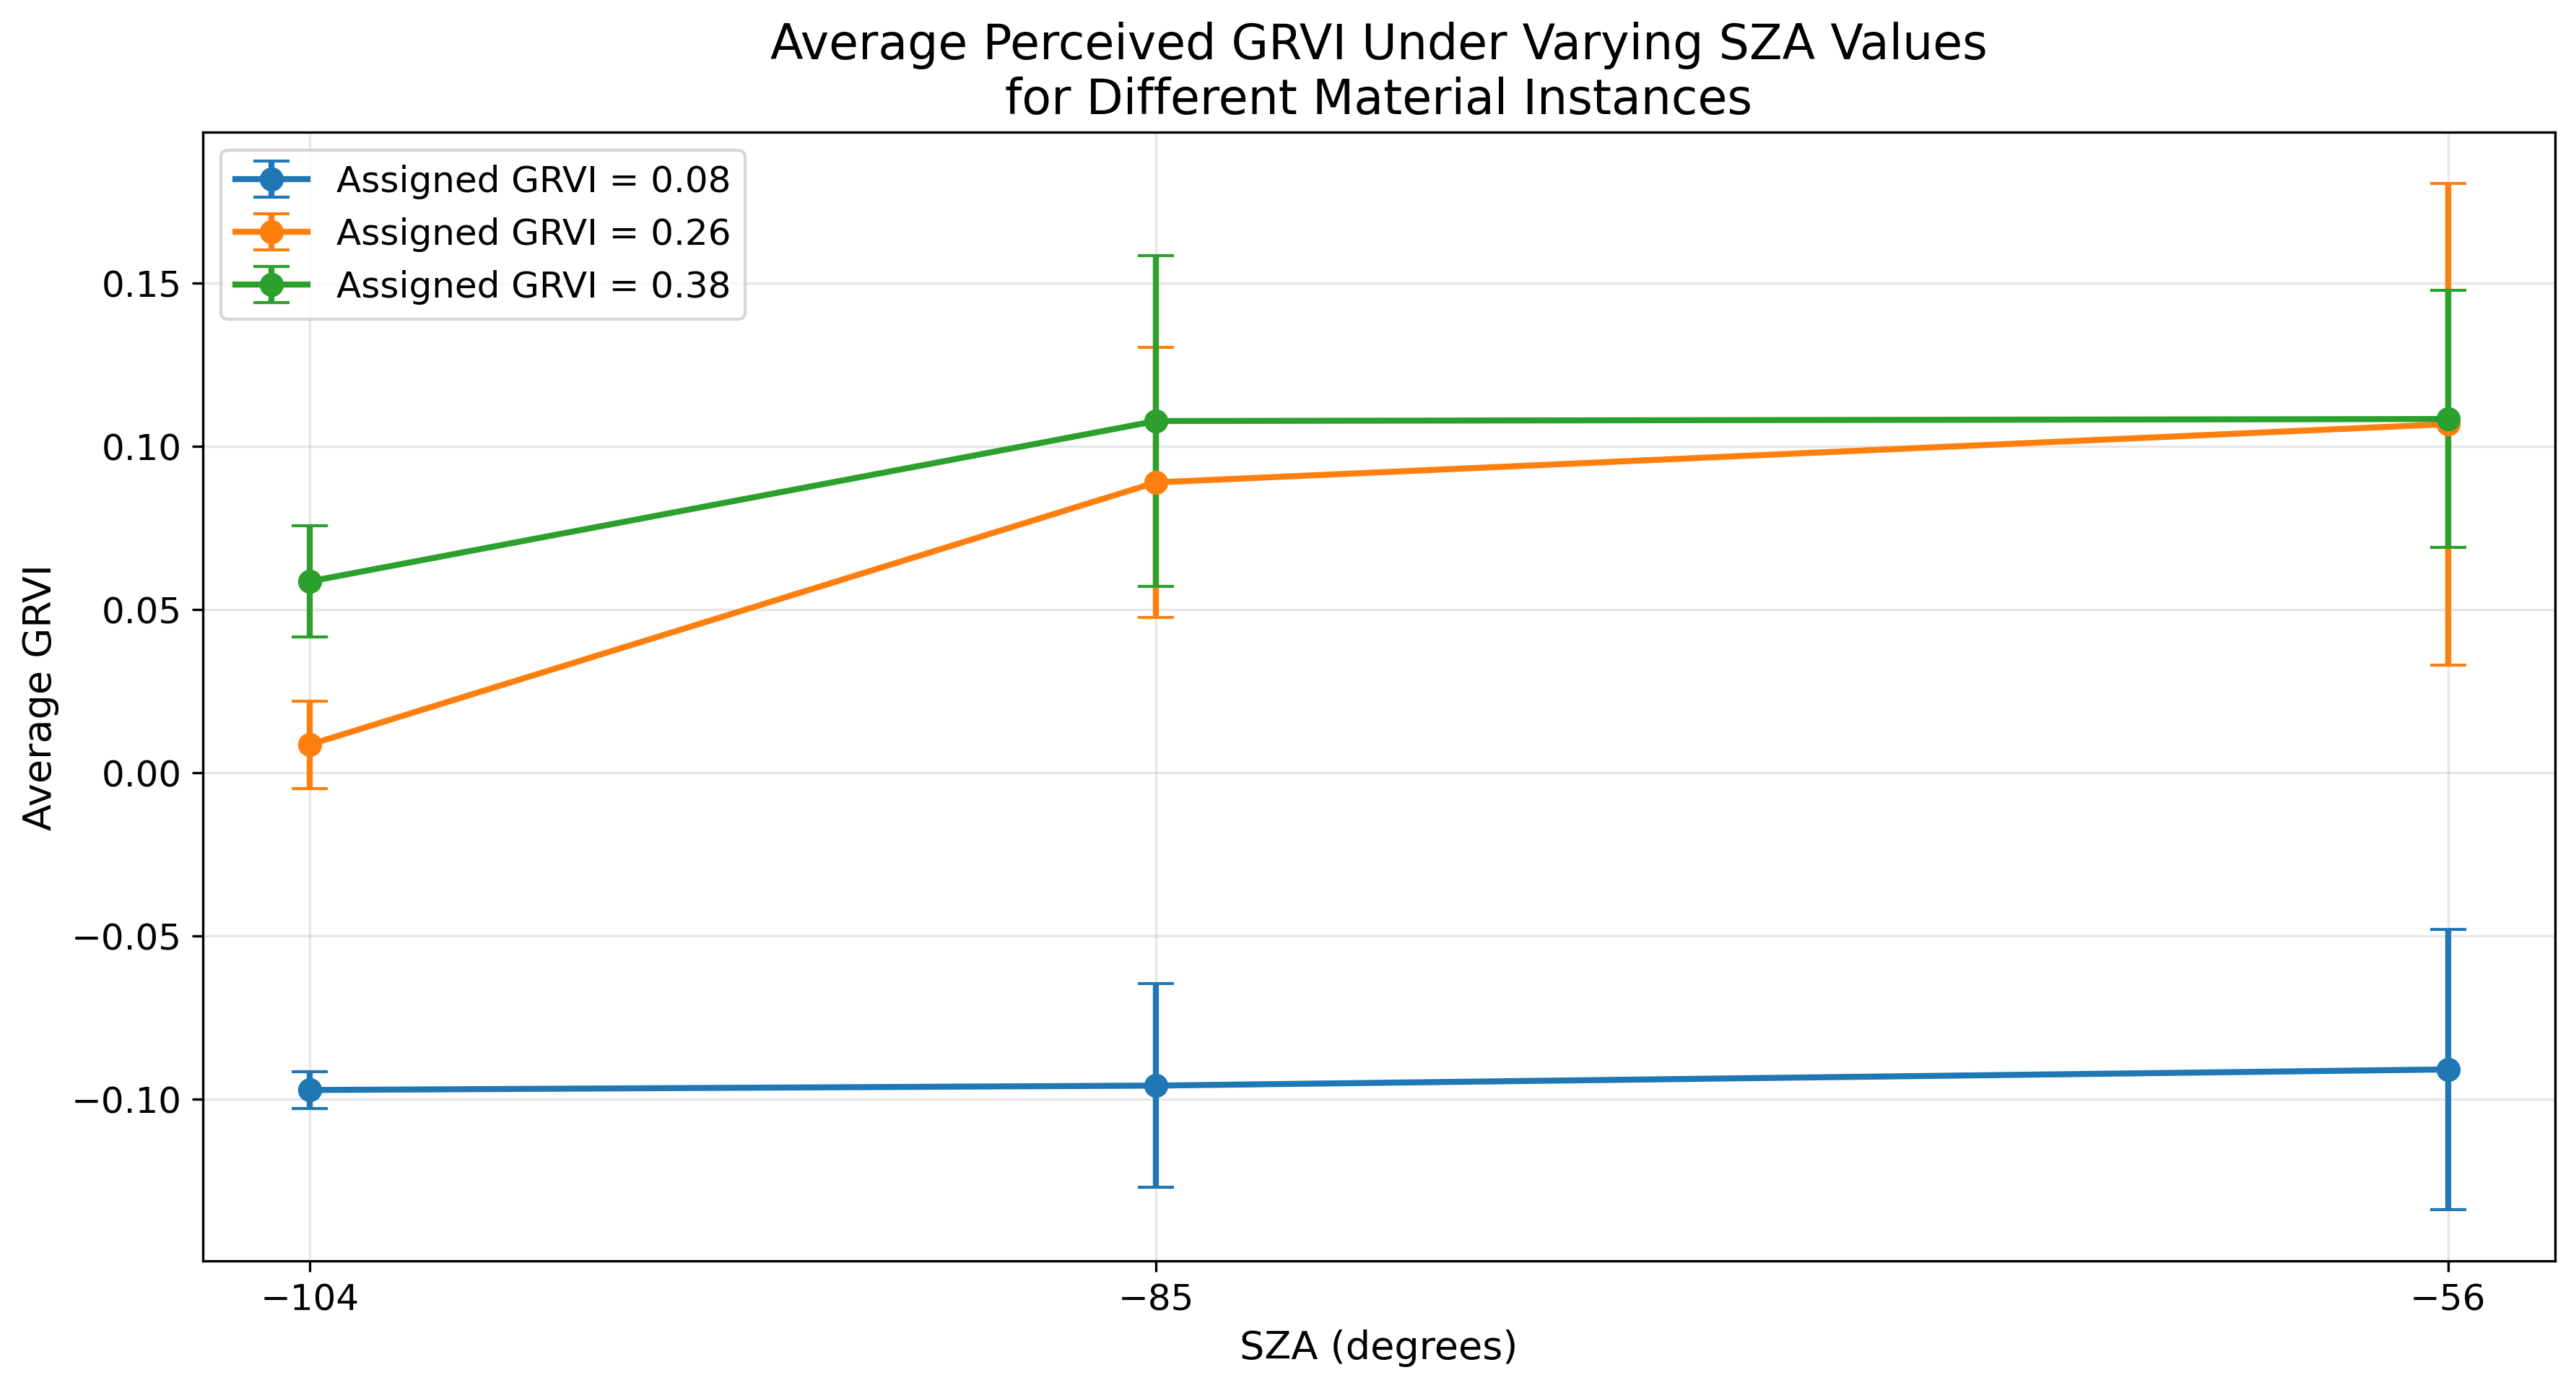
\includegraphics[width=1\linewidth]{images/grvi_vs_sza.png}
    \caption{Average perceived GRVI calculated for different SZA values and different materials. Vertical lines represent standard deviation.}
    \label{gloomy-diff-mats-and-sza}
\end{figure}

Overall, the findings suggest that the presence of shadows introduces significant distortions in the perceived GRVI values, affecting both their accuracy and consistency. The persistence of these deviations after outlier removal indicates that they cannot be attributed solely to isolated measurements, but rather reflect systematic effects associated with shaded conditions. Although the individual contribution of each identified factor remains difficult to isolate, the results demonstrate that shadows constitute an important source of GRVI measurement error and therefore justify their inclusion among the factors that the proposed correction models aim to address.


%note for later: REALLY need to find photos from the dataset with trees and shadows etc


\subsection{Front - Back}
!!!! some things about the front back thing + the grvi maps 



% Based on the problem they aim to tackle, there were two kinds of ML models developed. The first one aimed to tackle just the error introduced by the measuring media and conditions (the assumption of isotropic BDRF, non properly calibrated sensors, the variations caused by the different illumination scenarios etc.) and therefore was not trained to the half of the dataset that includes shadows. The second aimed to assess all sources of errors mentioned above, plus the inclusion of tree shadows.

%Another discrimination of the ML models that were developed regarded the selected ground truth. On the first case, four additional renders were performed, two for each render direction (start of spline to end of spline and the opposite). All four renders were performed under simulated overcast lighting, since overcast lighting eliminates the errors introduced by either BDRF anisotropy or shadows and all four were performed with a SZA of 20. Among the two renders corresponding to each direction, one was performed with a green-band illuminance of 322 and one with 1020, allowing the selection of the most suitable between the two (the criteria of the selection are analytically described in the next chapter). On the second case, the target GRVI of the models was the inherent GRVI of the material assigned to each plant mesh, with the estimation of which material was assigned to each depicted plant in the frame using the stored SCC coordinates.